\documentclass[11pt]{article}

\usepackage[margin=1in]{geometry}
\usepackage{amsmath,amssymb,amsthm}
\usepackage{graphicx}
\usepackage{booktabs}
\usepackage{xcolor}
\usepackage[authoryear,round]{natbib}
\usepackage{hyperref}
\usepackage{setspace}
\onehalfspacing

% figures are shared with the slides
\graphicspath{{../slides/figs/}}

% drafting notes: \todo{...} prints in red; delete before circulating
\newtheorem{proposition}{Proposition}
\newtheorem{corollary}{Corollary}
\newtheorem{lemma}{Lemma}
\renewcommand{\thelemma}{A.\arabic{lemma}}
\theoremstyle{definition}
\newtheorem{definition}{Definition}

\newcommand{\todo}[1]{{\color{red}\small[\textbf{TODO:} #1]}}
\newcommand{\note}[1]{{\color{gray}\small[#1]}}

\title{Time to Build and the Macroeconomy\thanks{\todo{acknowledgements}}}
\author{Samuel Zhao\\University of Chicago}
\date{\today}

\begin{document}
\maketitle

% =====================================================================
\begin{abstract}
\noindent
Production takes time: labour hired today becomes goods sold weeks or months later. We ask how this
changes monetary policy. Producers choose how long to produce, and industry inventory-to-cost
ratios imply production lags of up to a year across 269 goods industries. In the competitive economy,
durations are locally invariant to small shocks, growth and higher interest rates shorten them,
and time to build shifts the response to productivity shocks across dates without changing its
total. We then add household saving and a rigid nominal wage, and compare optimal policy under
commitment with the same economy without time to build. Time to build reverses the optimal response
to a productivity shock, cutting the rate to zero where the standard model hikes. It spreads policy
over several months and raises the gain from policy ten- to fifty-fold, while lowering it for demand
shocks. It also changes which shocks take the economy to the zero lower bound: supply shocks rather
than demand shocks. Warning about a shock is valuable only with time to build, and only because firms
can re-plan production.
\end{abstract}

\noindent\textbf{JEL:} E31, E43, E52, E22, E23.\quad
\textbf{Keywords:} time to build, optimal monetary policy, cost channel, news shocks, production commitment.

\newpage
% =====================================================================
\section{Introduction}\label{sec:intro}

Production takes time. A manufacturer hires workers and buys materials today and sells the
finished goods weeks or months later. Across six-digit US goods industries, inventories held per
dollar of annual cost of goods sold imply that the median unit of cost waits about two and a half
months before it is sold, and some industries wait more than a year (Antr\`as and Tubdenov, 2025).
Standard New Keynesian models abstract from this: output is produced in the period it is sold, and
monetary policy works through households' intertemporal choices. This paper asks whether time to
build changes how monetary policy should be conducted.

\paragraph{What we do.}
Each producer hires labour now for delivery later, and chooses how long to produce. Waiting is
physically costly but raises output per worker, and producers differ in how much it does. The
interest rate is the cost of carrying goods in production. We calibrate each producer's
time-to-build productivity so that its steady-state duration matches its industry's
inventory-to-cost ratio. We first study the competitive economy without household saving, where
the interest rate is a cost of production and nothing else. We then add nominal bonds and a rigid
nominal wage, and solve for the interest-rate path chosen by a planner with commitment. For
tractability, durations are held at their steady-state values in the policy analysis, so
production lags are fixed but heterogeneous across producers. Every policy experiment is compared
with the same economy without time to build.

\paragraph{Main results.}
\begin{enumerate}
  \item \textbf{The competitive economy.} Durations are locally invariant to small shocks, and
        growth or a higher interest rate shortens them (Propositions~\ref{prop:growth}
        and~\ref{prop:local}). To first order, time to build moves the response to a productivity
        shock across dates without changing its cumulative size, while an interest-rate rise
        lowers cumulative output in proportion to the mean lag (Corollary~\ref{cor:first}). Once
        households can save and the wage is flexible, the nominal rate is neutral
        (Proposition~\ref{prop:neutral}), so policy needs a nominal rigidity.
  \item \textbf{Time to build changes the sign and timing of optimal policy.} After an
        unexpected productivity fall, the optimal rate is cut to zero on impact. Without time to
        build, it is raised for one month, to 25\% annualised. It stays away from the peg for seven
        months rather than one. With news, the planner starts moving eleven months before the shock
        rather than three.
  \item \textbf{Policy matters more for supply shocks and less for demand shocks.} Time to build
        makes a productivity shock more than thirty times as costly under the peg, and raises the
        gain from optimal policy by a factor of 10--50. Committed production absorbs a demand shock,
        and the gain from policy is smaller.
  \item \textbf{The zero lower bound binds for supply shocks.} Because the optimal response to a
        productivity fall becomes a cut, time to build takes the economy to the zero bound after
        supply shocks, and the bound limits policy to removing a third of the loss. Without time to
        build, the bound binds after demand shocks instead, as in the standard model.
  \item \textbf{Warning is valuable only with time to build, and only through firms.} One period
        of warning about a productivity shock triples the gain from policy (0.12 $\to$ 0.37); without
        time to build it does not help. If production cannot be re-planned, earlier information
        is worth exactly nothing.
  \item \textbf{Who should know.} With rigid wages, public news of a supply shock triggers a
        hiring rush, so households are better off if only the planner knows. Public news of a
        demand shock lets production adjust, so households are better off if everyone knows.
\end{enumerate}

\paragraph{Related literature.}
\todo{fill citations}
\begin{itemize}
  \item Time to build and production lags: Kydland--Prescott; \ldots
  \item Cost channel of monetary policy: Barth--Ramey; Christiano--Eichenbaum--Evans; Ravenna--Walsh; \ldots
  \item Optimal policy in NK models: Woodford; Gal\'{i}; Benigno--Woodford; \ldots
  \item Wage rigidity: Erceg--Henderson--Levin; \ldots
  \item News shocks and forward guidance: Beaudry--Portier; Del Negro--Giannoni--Patterson; \ldots
  \item Value of public information: Hirshleifer; Morris--Shin; \ldots
\end{itemize}

\paragraph{Roadmap.}
Section~\ref{sec:model} presents the model, Section~\ref{sec:calib} the calibration,
Section~\ref{sec:mech} how shocks propagate, Section~\ref{sec:policy} the policy problem,
Section~\ref{sec:results} how optimal policy differs with and without time to build, and
Section~\ref{sec:concl} concludes.

% =====================================================================
\section{Model}\label{sec:model}

Time is discrete, $t=0,1,2,\dots$, and there is no capital. A representative household consumes
and supplies labour; a competitive final-good firm aggregates intermediate goods; and $F+1$
perfectly competitive intermediate-good producers, indexed by $j=0,\dots,F$, choose both how much
labour to hire and how long production takes. Producers differ in how productive time spent in
production is. Labour is the numeraire, $W_t=1$. The interest rate $i_t$ is the one-period rate on
claims denominated in labour; producers discount at it, and we take its path as given. The other
exogenous processes are aggregate productivity $A_t$ and the productivity of time in production
$B_t$. This section characterises the competitive equilibrium with a flexible wage and no
household saving. Section~\ref{sec:policy} adds household bonds and a rigid nominal wage for the
policy analysis.

% ---------------------------------------------------------------------
\subsection{Households}\label{sec:hh}

The household chooses consumption $C_t$ and labour $L_t$ to solve
\begin{equation}\label{eq:hh}
  \max_{\{C_t,L_t\}}\;\sum_{t=0}^{\infty}\beta^t
     \Bigl(\frac{C_t^{1-\sigma}}{1-\sigma}-\chi\frac{L_t^{1+\eta}}{1+\eta}\Bigr)
  \quad\text{s.t.}\quad P_tC_t=W_tL_t+\Pi_t ,
\end{equation}
where $P_t$ is the price of the final good in units of labour, $W_t=1$ the wage and $\Pi_t$ the profits
paid out by producers. The parameter $\sigma>0$ governs the curvature of consumption utility,
$\eta>0$ that of labour disutility, and $\chi>0$ scales labour disutility. The household cannot save,
so its problem is static, with first-order condition
\begin{equation}\label{eq:foc}
  \chi L_t^{\eta}C_t^{\sigma}=\frac{W_t}{P_t}=\frac{1}{P_t} .
\end{equation}
The real wage is $1/P_t$. Neither $\beta$ nor the interest rate enters the household's choices.

% ---------------------------------------------------------------------
\subsection{Final good}\label{sec:final}

Let $\tilde y_{j,\tau}$ denote the quantity of intermediate good $j$ available at date $\tau$. The
final good is produced competitively with the CES aggregator
\begin{equation}\label{eq:ces}
  Y_\tau=\Bigl(\sum_{j=0}^{F}\tilde y_{j,\tau}^{\frac{\varepsilon-1}{\varepsilon}}\Bigr)^{\frac{\varepsilon}{\varepsilon-1}},
  \qquad\varepsilon>1 .
\end{equation}
The final-good firm solves $\max_{\{\tilde y_{j,\tau}\}}P_\tau Y_\tau-\sum_j p_{j,\tau}\tilde y_{j,\tau}$, giving
\begin{equation}\label{eq:demand}
  p_{j,\tau}=P_\tau\Bigl(\frac{Y_\tau}{\tilde y_{j,\tau}}\Bigr)^{1/\varepsilon},\qquad
  P_\tau=\Bigl(\sum_{j=0}^{F}p_{j,\tau}^{\,1-\varepsilon}\Bigr)^{\frac{1}{1-\varepsilon}} .
\end{equation}

% ---------------------------------------------------------------------
\subsection{Intermediate-good producers}\label{sec:firms}

\paragraph{Technology.}
If producer $j$ hires $l_{j,t}$ units of labour at $t$ and completes production at
$\tau\in\{t,\dots,t+T_j\}$, output delivered at $\tau$ is
\begin{equation}\label{eq:tech}
  y_{j,\tau|t}=\kappa^{\tau-t}\,\bigl(\tau-t+B_tN_j\bigr)\,A_t\,l_{j,t},\qquad\kappa\in(0,1).
\end{equation}
$\kappa^{\tau-t}$ is the physical cost of time in production; $\tau-t+B_tN_j$ is the productivity gain
from time in production, with $N_j$ producer $j$'s time-to-build productivity and $B_t$ an aggregate
shifter. Productivity is dated at the start of production. The good available at $\tau$ adds up
batches started at different dates,
\begin{equation}\label{eq:vintage}
  \tilde y_{j,\tau}=\sum_{t\le\tau}y_{j,\tau|t} .
\end{equation}

\paragraph{Problem.}
Let $\delta_s\equiv1/(1+i_s)$ be the discount factor between $s$ and $s+1$, and
$Q_t\equiv\prod_{s=0}^{t-1}\delta_s$. Producer $j$ chooses, for each start date $t$, labour
$l_{j,t}$ and a completion date $\tau_{j,t}$ to maximise
\begin{equation}\label{eq:firmprob}
  \max_{\{l_{j,t},\,\tau_{j,t}\}}\;\sum_{t\ge0}\Bigl(Q_{\tau_{j,t}}\,p_{j,\tau_{j,t}}\,y_{j,\tau_{j,t}|t}
     -Q_t\,l_{j,t}\Bigr),
  \qquad t\le\tau_{j,t}\le t+T_j .
\end{equation}
Producers pay wages when production starts and are paid on delivery, so $i_t$ is the cost of
carrying goods in production.

\paragraph{Optimality.}
The value at $t$ of one unit of labour sent to completion date $\tau$ is
\begin{equation}\label{eq:value}
  v_{j,t}(\tau)\equiv p_{j,\tau}\Bigl(\prod_{s=t}^{\tau-1}\delta_s\Bigr)\kappa^{\tau-t}\bigl(\tau-t+B_tN_j\bigr)A_t .
\end{equation}
With constant returns and free entry, $\max_\tau v_{j,t}(\tau)\le 1$, with equality whenever
$l_{j,t}>0$, and labour is sent only to the completion dates that attain the maximum:
\begin{equation}\label{eq:zeroprofit}
  \tau_{j,t}\in\arg\max_{\tau}v_{j,t}(\tau),\qquad v_{j,t}(\tau_{j,t})=1\ \text{ if } l_{j,t}>0 .
\end{equation}
Each batch earns zero profit in present value at the rate $i_t$. Profits paid out at $t$ are the cash
flow $\Pi_t=\sum_jp_{j,t}\tilde y_{j,t}-L_t$: the return on goods in production. It is positive in the
steady state and can turn negative when hiring surges, in which case the household finances it.
Because the household cannot save, it does not price this cash flow: producers' discounting is set
by $i_t$, not by the household's marginal rate of substitution.

% ---------------------------------------------------------------------
\subsection{Equilibrium}\label{sec:eq}

\begin{definition}[Equilibrium]\label{def:eq}
Given initial conditions $\{y_{j,\tau|t}\}_{t<0\le\tau}$ (goods already in production at date 0), a
sequence of interest rates $\{i_t\}_{t\ge0}$ and shocks $\{A_t,B_t\}_{t\ge0}$, an equilibrium
is a sequence of prices $\{P_t,\{p_{j,t}\}_{j}\}_{t\ge0}$, with $W_t=1$, and allocations
$\{C_t,Y_t,L_t,\{l_{j,t},\tilde y_{j,t},\{y_{j,t|s}\}_{s\le t},\tau_{j,t}\}_{j}\}_{t\ge0}$ such that
\begin{enumerate}
  \item the household maximises \eqref{eq:hh}, given $\{P_t,\Pi_t\}$;
  \item the final-good firm maximises profits, given $\{P_t,\{p_{j,t}\}_j\}$;
  \item each producer solves \eqref{eq:firmprob}, given $\{i_t,\{p_{j,s}\}_{s\ge t}\}$;
  \item markets clear: $C_t=Y_t$, $L_t=\sum_jl_{j,t}$ and $\tilde y_{j,t}=\sum_{s\le t}y_{j,t|s}$;
  \item the economy returns to the steady state: $\lim_{t\to\infty}(C_t,L_t)=(C,L)$.
\end{enumerate}
\end{definition}

\noindent The budget constraint holds by the definition of $\Pi_t$ and $C_t=Y_t$. The terminal
condition is needed because hiring is forward-looking: labour hired at $t$ is set by demand at the
delivery dates.

% ---------------------------------------------------------------------
\subsection{Steady state}\label{sec:ss}

In the steady state $A_t=A$, $B_t=B$ and $i_t=i$, so $\delta_s=\delta\equiv1/(1+i)$. Define
producer $j$'s \emph{effective productivity} of a duration $\Delta$,
\begin{equation}\label{eq:effprod}
  z_j(\Delta)\equiv(\kappa\delta)^{\Delta}\bigl(\Delta+BN_j\bigr)A .
\end{equation}
By \eqref{eq:value}, producer $j$ chooses the duration that maximises $z_j(\Delta)$. Treating
$\Delta$ as continuous, the first-order condition gives
\begin{equation}\label{eq:ssdur}
  \Delta_j^{SS}=\max\Bigl\{-\frac{1}{\log(\delta\kappa)}-BN_j,\;0\Bigr\},
\end{equation}
with the integer choice the better of $\lfloor\Delta_j^{SS}\rfloor$ and $\lceil\Delta_j^{SS}\rceil$.
Higher $\delta\kappa$ lengthens production; higher $N_j$ shortens it. Heterogeneity in $N_j$
generates a distribution of durations across producers. Write $\tau_j\equiv\Delta_j^{SS}$ and
$z_j\equiv z_j(\tau_j)$. Then
\begin{equation}\label{eq:ss}
  p_j=\frac{1}{z_j},\qquad \frac{1}{P}=\tilde A\equiv\Bigl(\sum_jz_j^{\varepsilon-1}\Bigr)^{\frac{1}{\varepsilon-1}},\qquad
  \tilde y_j=\Bigl(\frac{z_j}{\tilde A}\Bigr)^{\varepsilon}Y .
\end{equation}
Aggregating labour, output is proportional to hours, and labour supply pins down their level:
\begin{equation}\label{eq:ssL}
  Y=\Theta L,\quad \Theta\equiv\frac{\tilde A^{\varepsilon}}{\sum_jz_j^{\varepsilon-1}\delta^{\tau_j}},\qquad
  L=\Bigl(\frac{\tilde A}{\chi\,\Theta^{\sigma}}\Bigr)^{\frac{1}{\sigma+\eta}},\qquad C=Y .
\end{equation}
Since $\delta^{\tau_j}\le1$, $\Theta\ge\tilde A$: output per worker exceeds the real wage, and the
difference, $\Pi/P=(1-\tilde A/\Theta)Y$, is the return on goods in production.

Two sets of weights recur below. Producer $j$'s share of expenditure and its share of employment are
\begin{equation}\label{eq:weights}
  s_j\equiv\frac{p_j\tilde y_j}{PY}=\Bigl(\frac{z_j}{\tilde A}\Bigr)^{\varepsilon-1},\qquad
  \lambda_j\equiv\frac{l_j}{L}=\frac{s_j\delta^{\tau_j}}{\sum_ks_k\delta^{\tau_k}} .
\end{equation}
Employment shares discount long lags: a producer with a long lag pays its workers earlier, relative
to its sales, than one with a short lag. We write $\bar\tau_s\equiv\sum_js_j\tau_j$ and
$\bar\tau_\lambda\equiv\sum_j\lambda_j\tau_j$ for the mean lag under each set of weights. Then
$\bar\tau_\lambda\le\bar\tau_s$, strictly if $\delta<1$ and lags differ across producers
(Appendix~\ref{app:meanlags}).

% ---------------------------------------------------------------------
\subsection{Growth, interest rates and production duration}\label{sec:growth}

Suppose productivity grows at a constant rate, $A_t=(1+g)^tA_0$ with $g>-1$, while $B_t=B$ and
the interest rate is constant at $i$. Consider a balanced growth path: an equilibrium in which every
producer uses a constant duration, prices in units of labour fall at the rate of productivity growth,
$p_{j,t}A_t$ constant, and $C_t$ and $L_t$ grow at constant rates. On such a path the value of a worker
\eqref{eq:value} is proportional to $\bigl(\delta\kappa/(1+g)\bigr)^{\Delta}(\Delta+BN_j)$, so,
treating $\Delta$ as continuous,
\begin{equation}\label{eq:gdur}
  \Delta_j^{g}=\max\Bigl\{-\frac{1}{\log\bigl(\delta\kappa/(1+g)\bigr)}-BN_j,\;0\Bigr\} .
\end{equation}
Consumption grows at $1+g_C=(1+g)^{\frac{1+\eta}{\sigma+\eta}}$ and hours at
$(1+g)^{\frac{1-\sigma}{\sigma+\eta}}$.

\begin{proposition}[Growth, interest rates and production duration]\label{prop:growth}
Let $\tau_j(g,i)$ be producer $j$'s duration on the balanced growth path with growth rate $g$ and
interest rate $i$, and $\tau_j^{SS}=\tau_j(0,i)$. Every selection of $\tau_j(g,i)$ is nonincreasing in
$g$ and in $i$. In particular, $g>0$ implies $\tau_j(g,i)\le\tau_j^{SS}$ and $g<0$ implies
$\tau_j(g,i)\ge\tau_j^{SS}$.
\end{proposition}

\noindent The proof is in Appendix~\ref{app:pf_growth}. Durations depend on growth and the interest rate only
through $\delta\kappa/(1+g)$. Measured in labour, a good becomes cheaper as productivity grows, so a
good delivered later is worth less in terms of today's wage. Growth therefore raises the cost of time
in production in the same way as a higher interest rate.

% ---------------------------------------------------------------------
\subsection{Small shocks and fixed durations}\label{sec:small}

\begin{proposition}[Local invariance of time to build]\label{prop:local}
Suppose each $\tau_j$ is the unique maximiser of $z_j(\cdot)$. Consider a sequence $\{i_s,A_s,B_s\}$
equal to its steady-state values except at one date $t$. For sufficiently small deviations at $t$,
there exists an equilibrium in which $\tau_{j,s}=s+\tau_j$ for all producers $j$ and dates $s$.
\end{proposition}

\noindent The proof is in Appendix~\ref{app:pf_local}.

\medskip
\noindent Around the steady state the economy therefore behaves like one with exogenous
production lags $\tau_j$. With fixed durations, define output per unit of labour
$\zeta_{j,t}\equiv\kappa^{\tau_j}(\tau_j+B_tN_j)$, so that $y_{j,t+\tau_j|t}=\zeta_{j,t}A_tl_{j,t}$.
Zero profit \eqref{eq:zeroprofit} then gives the price of good $j$ delivered at $t\ge\tau_j$:
\begin{equation}\label{eq:price}
  p_{j,t}=\frac{\prod_{s=t-\tau_j}^{t-1}(1+i_s)}{\zeta_{j,t-\tau_j}\,A_{t-\tau_j}},
  \qquad
  P_t=\Biggl(\sum_j\Bigl[\frac{\prod_{s=t-\tau_j}^{t-1}(1+i_s)}{\zeta_{j,t-\tau_j}A_{t-\tau_j}}\Bigr]^{1-\varepsilon}\Biggr)^{\frac{1}{1-\varepsilon}}
  \quad(t\ge\max_j\tau_j).
\end{equation}
Prices in units of labour are set by costs alone: the interest rate over the production window and
productivity at the start. A higher interest rate raises the price level and lowers the real wage
$1/P_t$ for the next $\max_j\tau_j$ periods. It also changes relative prices, since it raises the
cost of long-lag goods by more. So the interest rate has real effects even though the wage is
flexible. Before $\max_j\tau_j$, goods from batches started before date 0 are in fixed supply,
and their prices are set by demand \eqref{eq:demand}.

% ---------------------------------------------------------------------
\subsection{First-order responses}\label{sec:firstorder}

We linearise the economy with fixed durations around the steady state, holding $B_t=B$. Hats denote
log deviations, and $\hat\imath_t\equiv\log(1+i_t)-\log(1+i)$. We consider \emph{anticipated} shocks:
every agent knows the shock before any batch affected by it has been started. Formally, we
linearise on $t\in\mathbb Z$, with all deviations vanishing as $t\to\pm\infty$. Define the
lag-generating function of employment and its reciprocal,
\begin{equation}\label{eq:Lambda}
  \Lambda(z)\equiv\sum_j\lambda_jz^{\tau_j},\qquad
  \Psi(z)\equiv\frac{1}{\sigma+\eta\Lambda(z)}=\sum_{k\ge0}\psi_kz^k .
\end{equation}
Let $\bar s_k\equiv\sum_{j:\tau_j=k}s_j$ be the expenditure share of goods with lag $k$, and
$\bar S_k\equiv\sum_{j:\tau_j\ge k}s_j$ the share with lag at least $k$.

\begin{corollary}[First-order responses]\label{cor:first}
Suppose $\sigma+\eta\Lambda(z)\neq0$ for $|z|\le1$; a sufficient condition is
$\sigma>\eta(1-2\lambda_0)$. Then the linearised economy has a unique bounded solution, and:
\begin{enumerate}
  \item[(a)] \emph{Prices.} $\hat p_{j,t}=\sum_{s=t-\tau_j}^{t-1}\hat\imath_s-\hat A_{t-\tau_j}$ and
        $\hat P_t=\sum_js_j\hat p_{j,t}$. For a productivity shock $\hat A_{t_0}=a$,
        $\hat P_{t_0+k}=-\bar s_k\,a$ for $k\ge0$. For an interest-rate shock $\hat\imath_{t_0}=\iota$,
        $\hat P_{t_0+k}=\bar S_k\,\iota$ for $k\ge1$, and $\hat P_t=0$ for $t\le t_0$.
  \item[(b)] \emph{Output.} Output satisfies
        $\sigma\hat Y_t+\eta\sum_j\lambda_j\hat Y_{t+\tau_j}=X_t$, so
        \begin{equation}\label{eq:Yfirst}
          \hat Y_t=\sum_{k\ge0}\psi_k\,X_{t+k},\qquad
          X_t\equiv-\hat P_t+\eta\hat A_t+\eta\varepsilon\sum_j\lambda_j\bigl(\hat p_{j,t+\tau_j}-\hat P_{t+\tau_j}\bigr),
        \end{equation}
        and hours are
        $\hat L_t=\sum_j\lambda_j\bigl[\hat Y_{t+\tau_j}-\varepsilon(\hat p_{j,t+\tau_j}-\hat P_{t+\tau_j})\bigr]-\hat A_t$.
  \item[(c)] \emph{Cumulative output.} For absolutely summable shocks,
        \begin{equation}\label{eq:cum}
          \sum_t\hat Y_t=\frac{1+\eta}{\sigma+\eta}\sum_t\hat A_t
          -\frac{\bar\tau_s+\eta\varepsilon(\bar\tau_s-\bar\tau_\lambda)}{\sigma+\eta}\sum_t\hat\imath_t .
        \end{equation}
  \item[(d)] \emph{No time to build.} If $\tau_j=0$ for all $j$, then
        $\hat Y_t=\frac{1+\eta}{\sigma+\eta}\hat A_t$ and the interest rate has no effect.
\end{enumerate}
\end{corollary}

\noindent The proof is in Appendix~\ref{app:pf_first}. The output equation in (b) comes from labour supply,
$\eta\hat L_t+\sigma\hat Y_t=-\hat P_t$, with hours set by demand at the delivery dates. Output
today depends on output in the future, because labour hired today produces goods delivered later.

Part (c) says that, for a productivity shock, time to build moves the response across dates without
changing its total. The cumulative response, $(1+\eta)/(\sigma+\eta)$, is the same as without time
to build. The timing differs. Prices fall as the affected batches are delivered, in proportion to
the expenditure share of each lag, $\bar s_k$. Hours rise on the shock date, as producers hire to
exploit the higher productivity. The household cannot save, so by \eqref{eq:foc} it supplies the
extra hours only if consumption falls. Output therefore \emph{falls} on the shock date and rises at
later delivery dates.

An interest-rate rise is a cost shock. It raises the price of every good whose production window
spans the date of the rise. Goods with lag at least $k$, a share $\bar S_k$ of expenditure, are
still priced higher $k$ periods later. Cumulative output falls in proportion to the mean lag. Since
$\bar\tau_\lambda\approx\bar\tau_s$ when $\delta$ is close to one, a one-period rise of $\iota$
lowers cumulative output by about $\bar\tau_s\iota/(\sigma+\eta)$. That is the effect of a fall
in productivity of $\bar\tau_s\iota/(1+\eta)$.

In the calibration of Section~\ref{sec:calib}, $\bar\tau_s=2.44$, $\bar\tau_\lambda=2.44$ and
$\lambda_0=0.007$, so the condition in Corollary~\ref{cor:first} holds. With $\sigma=\eta=2$ and
$\varepsilon=5$, the cumulative responses are $0.75$ to productivity and $-0.62$ to the interest rate
(per unit of $\hat\imath$).

\paragraph{Unexpected shocks.} If the shock is revealed at date 0, batches already in production
are committed, and for $t<\max_j\tau_j$ part of the price level is set by demand for goods in
fixed supply. The linear system then has date-dependent coefficients before $\max_j\tau_j$
(Appendix~\ref{app:pf_first}), and \eqref{eq:cum} no longer applies. A productivity shock still
triggers a hiring rush at date 0. Now, however, the prices of committed goods fall, which raises
the real wage, so consumption barely moves. Output also does not fall ahead of the shock. In the
calibration the cumulative output response is $2.05$, compared with $0.75$ when the shock is
anticipated.

\paragraph{Household saving.} The interest rate has real effects in this section because the
household cannot save. Section~\ref{sec:policy} shows that with nominal bonds and a flexible wage the
nominal rate is neutral (Proposition~\ref{prop:neutral}). The policy analysis therefore adds a rigid
nominal wage.

% =====================================================================
\section{Calibration}\label{sec:calib}

\paragraph{Data and period length.}
Each producer is a six-digit NAICS goods-producing industry, $F+1=269$ in total. For each industry we
observe the ratio of inventories to annual cost of goods sold, from Antr\`as and Tubdenov (2025).
We read inventories as goods in production: the ratio times 365 is the number of days a unit of cost
stays in the firm before the good is sold. One period is a month of 30 days, so industry $j$'s
duration in the data is $\tau_j^{data}=365\times(\text{inventory}/\text{COGS})_j/30$ months. It has
mean 2.9 months, median 2.6, and ranges from 0.4 to 12.9. All rates below are monthly.

\paragraph{Durations.}
We set $B=1$ and choose each $N_j$ so that the continuous steady-state duration \eqref{eq:ssdur}
equals the data,
\[
  N_j=-\frac{1}{\log(\delta\kappa)}-\tau_j^{data}.
\]
The model's duration $\tau_j$ is then the better of $\lfloor\tau_j^{data}\rfloor$ and
$\lceil\tau_j^{data}\rceil$ (Appendix~\ref{app:discrete}). $N_j$ ranges from 2.0 to 14.5, so output per
worker is positive at every duration. Figure~\ref{fig:lags} shows the resulting distribution.
Durations range from 0 to 13 months, and 82\% of expenditure is on goods with lags of one to three
months. The mean lag is $\bar\tau_s=2.44$ months weighted by expenditure and $\bar\tau_\lambda=2.44$
weighted by employment; the two weights are almost identical because $\delta$ is close to one.

\paragraph{The cost of time.}
$\kappa$ governs how durations respond to the interest rate: by \eqref{eq:ssdur},
$\partial\Delta_j^{SS}/\partial\log\delta=1/(\log\delta\kappa)^2$ for every interior producer. Antr\`as and Tubdenov (2025, Table 5) regress the average period of
production in U.S.\ manufacturing on the cost of capital. They find a coefficient of $-0.090$ (s.e.\
0.007), stable at $-0.088$ to $-0.090$ across specifications: when the log cost of capital rises by one,
the period of production falls by 0.090 years, about 33 days. In our model the cost of capital is the
interest rate $i$, at which producers discount and finance goods in production. A one-month
(30-day) fall in durations therefore corresponds to a rise in $\log i$ of $(30/365)/0.090=0.913$, from
the steady-state rate of 0.327\% to $0.327\%\times e^{0.913}=0.816\%$ per month. Given $\kappa$, each
$N_j$ is set so that producer $j$'s duration at the steady-state rate matches the data. We then
grid-search over $\kappa$ for the value at which the mean absolute change in durations between the
two rates equals one month. This gives $\kappa=0.938$.

\paragraph{Other parameters.}
The steady-state rate is $i=0.327\%$ per month, 4\% a year. The elasticity of substitution is $\varepsilon=5$,
consumption curvature and the inverse Frisch elasticity are $\sigma=\eta=2$, and $\chi=1$ is a
normalisation. The household's $\beta$ does not affect the equilibrium of Section~\ref{sec:model};
for welfare we set $\beta=\delta$. Table~\ref{tab:calib} collects the values.

\begin{table}[h]
  \centering
  \caption{Calibration (one period $=$ one month of 30 days)}\label{tab:calib}
  \small
  \begin{tabular}{llll}
    \toprule
    & Parameter & Value & Target or source \\
    \midrule
    $F+1$ & producers & 269 & NAICS-6 goods industries \\
    $\tau_j^{data}$ & duration in the data & 0.4--12.9 (mean 2.9) & Antr\`as--Tubdenov (A--T, 2025) \\
    $N_j$ & time-to-build productivity & 2.0 to 14.5 & $\Delta_j^{SS}=\tau_j^{data}$ \\
    $B$ & aggregate shifter & 1 & normalisation \\
    $\kappa$ & physical cost of time & 0.938 & cost-of-capital response, A--T \\
    $i$ & interest rate & 0.327\% per month & 4\% a year; $\delta=0.9967$ \\
    $\varepsilon$ & elasticity of substitution & 5 & \\
    $\sigma$ & consumption curvature & 2 & \\
    $\eta$ & inverse Frisch elasticity & 2 & \\
    $\chi$ & labour disutility & 1 & normalisation \\
    \midrule
    \multicolumn{4}{l}{\emph{Implied}}\\
    $\tau_j$ & model durations & 0--13 & \\
    $\bar\tau_s,\ \bar\tau_\lambda$ & mean lag (exp., emp.) & 2.44, 2.44 & \\
    $\lambda_0$ & employment share with $\tau_j=0$ & 0.007 & \\
    $\Pi/(PY)$ & profits / output & 0.8\% & $1-\tilde A/\Theta$ \\
    \bottomrule
  \end{tabular}
\end{table}

\begin{figure}[h]
  \centering
  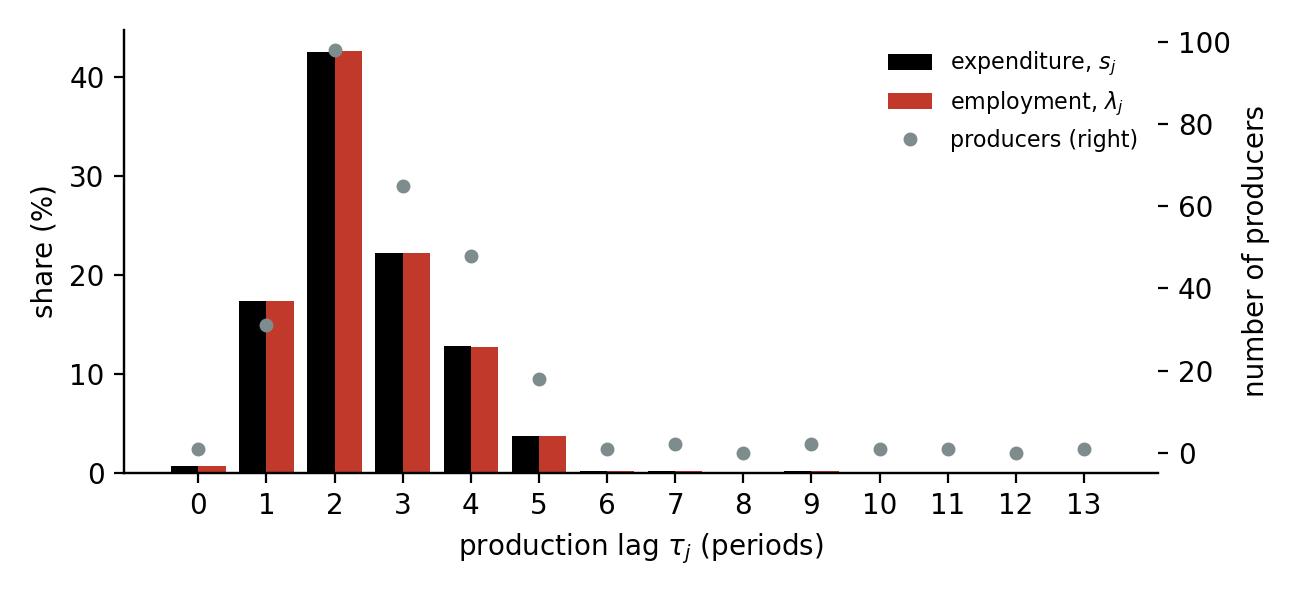
\includegraphics[width=0.8\textwidth]{ce_lags.png}
  \caption{Distribution of production lags. Bars: expenditure and employment shares by lag
  (left axis). Dots: number of producers (right axis).}
  \label{fig:lags}
\end{figure}

% =====================================================================
\section{Shock propagation in the competitive economy}\label{sec:mech}

This section shows how shocks propagate in the competitive economy of Section~\ref{sec:model}: no
saving, a flexible wage, and durations fixed at their steady-state values. We solve the nonlinear model
under perfect foresight. We compare three cases:
\begin{itemize}
  \item \emph{anticipated}: the shock is known from well before any affected batch is started (we
        announce it 50 months ahead);
  \item \emph{unexpected}: the shock is revealed on the date it hits, and batches already in production
        are committed;
  \item \emph{no time to build}: $\tau_j=0$ for all $j$, with the same $\zeta_j$.
\end{itemize}
Throughout, the price level is measured in units of labour, so a fall in $P_t$ is a rise in the real
wage. Profits are cash flow, $\Pi_t/P_t=Y_t-L_t/P_t$. Table~\ref{tab:prop} summarises the responses.

\subsection{A productivity shock}

Figure~\ref{fig:ce_tfp} shows a one-month 1\% rise in $A_t$ at date 0.

\paragraph{No time to build.} Output rises by $(1+\eta)/(\sigma+\eta)=0.75\%$ on impact and returns to
the steady state the next month. The price level falls by 1\%, one for one with costs.

\paragraph{Unexpected.} Labour hired at date 0 is more productive, but its output arrives only at
$\tau_j$. Hours rise by 2.7\% at date 0, while more than 99\% of the goods sold at date 0 come from
committed batches. Output therefore cannot rise, and the household supplies the extra hours only at a
higher real wage: the price level falls by 5.1\%. With output fixed and the wage bill higher, profits fall
by 8.2\% of steady-state output. From date 1 the productive batches are delivered: output rises by
1.0\%, 0.8\% and 0.3\% over the next three months. The response lasts as long as the longest lags;
the lower panels of Figure~\ref{fig:ce_tfp_bylag} trace it to each lag group. Cumulative output rises
by 2.1\%, almost three times the 0.75\% without time to build.

\paragraph{Anticipated.} The price level now moves only when the productive batches are delivered,
by $-\bar s_k$ at horizon $k$ (Corollary~\ref{cor:first}). Before the shock, prices and so the real
wage are unchanged, and labour supply reduces to $\eta\hat L_t=-\sigma\hat Y_t$. Hours and consumption
must move in opposite directions. Producers reshuffle hiring away from the dates just before the shock,
when hires would compete with the cheap batches started at date 0, and consumption rises: output is
1.3\% and 1.0\% above steady state two months and one month before the shock. On the shock date,
hiring jumps by 3.1\%, and since the real wage has not moved, consumption falls by 3.1\%. Output then rises
at the delivery dates as in the unexpected case. Cumulative output is 0.76\%, matching the linear
prediction of 0.75\% from Corollary~\ref{cor:first}: anticipation moves the response across dates but
leaves its total equal to the case without time to build.

\begin{figure}[h]
  \centering
  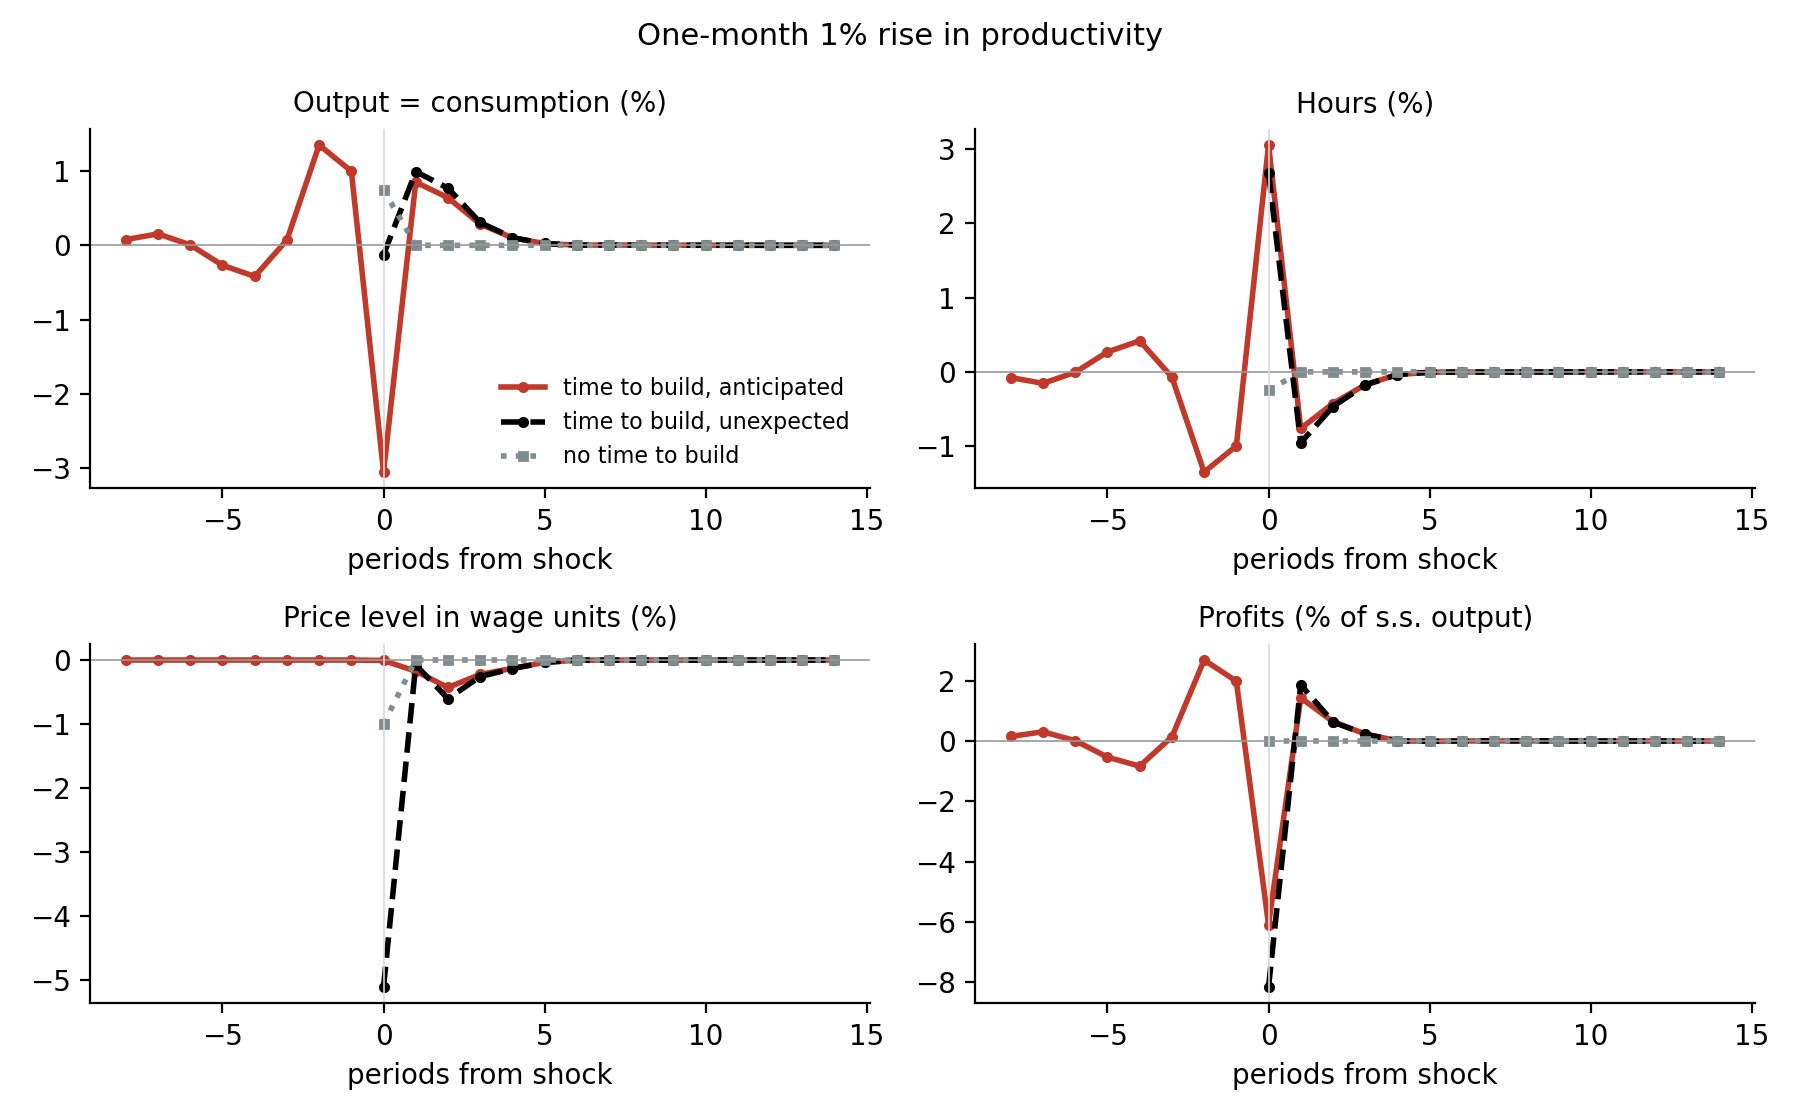
\includegraphics[width=\textwidth]{ce_tfp.png}
  \caption{A one-month 1\% rise in productivity at date 0. Competitive economy with fixed
  durations. Price level in units of labour; profits in \% of steady-state output.}
  \label{fig:ce_tfp}
\end{figure}

\begin{figure}[h]
  \centering
  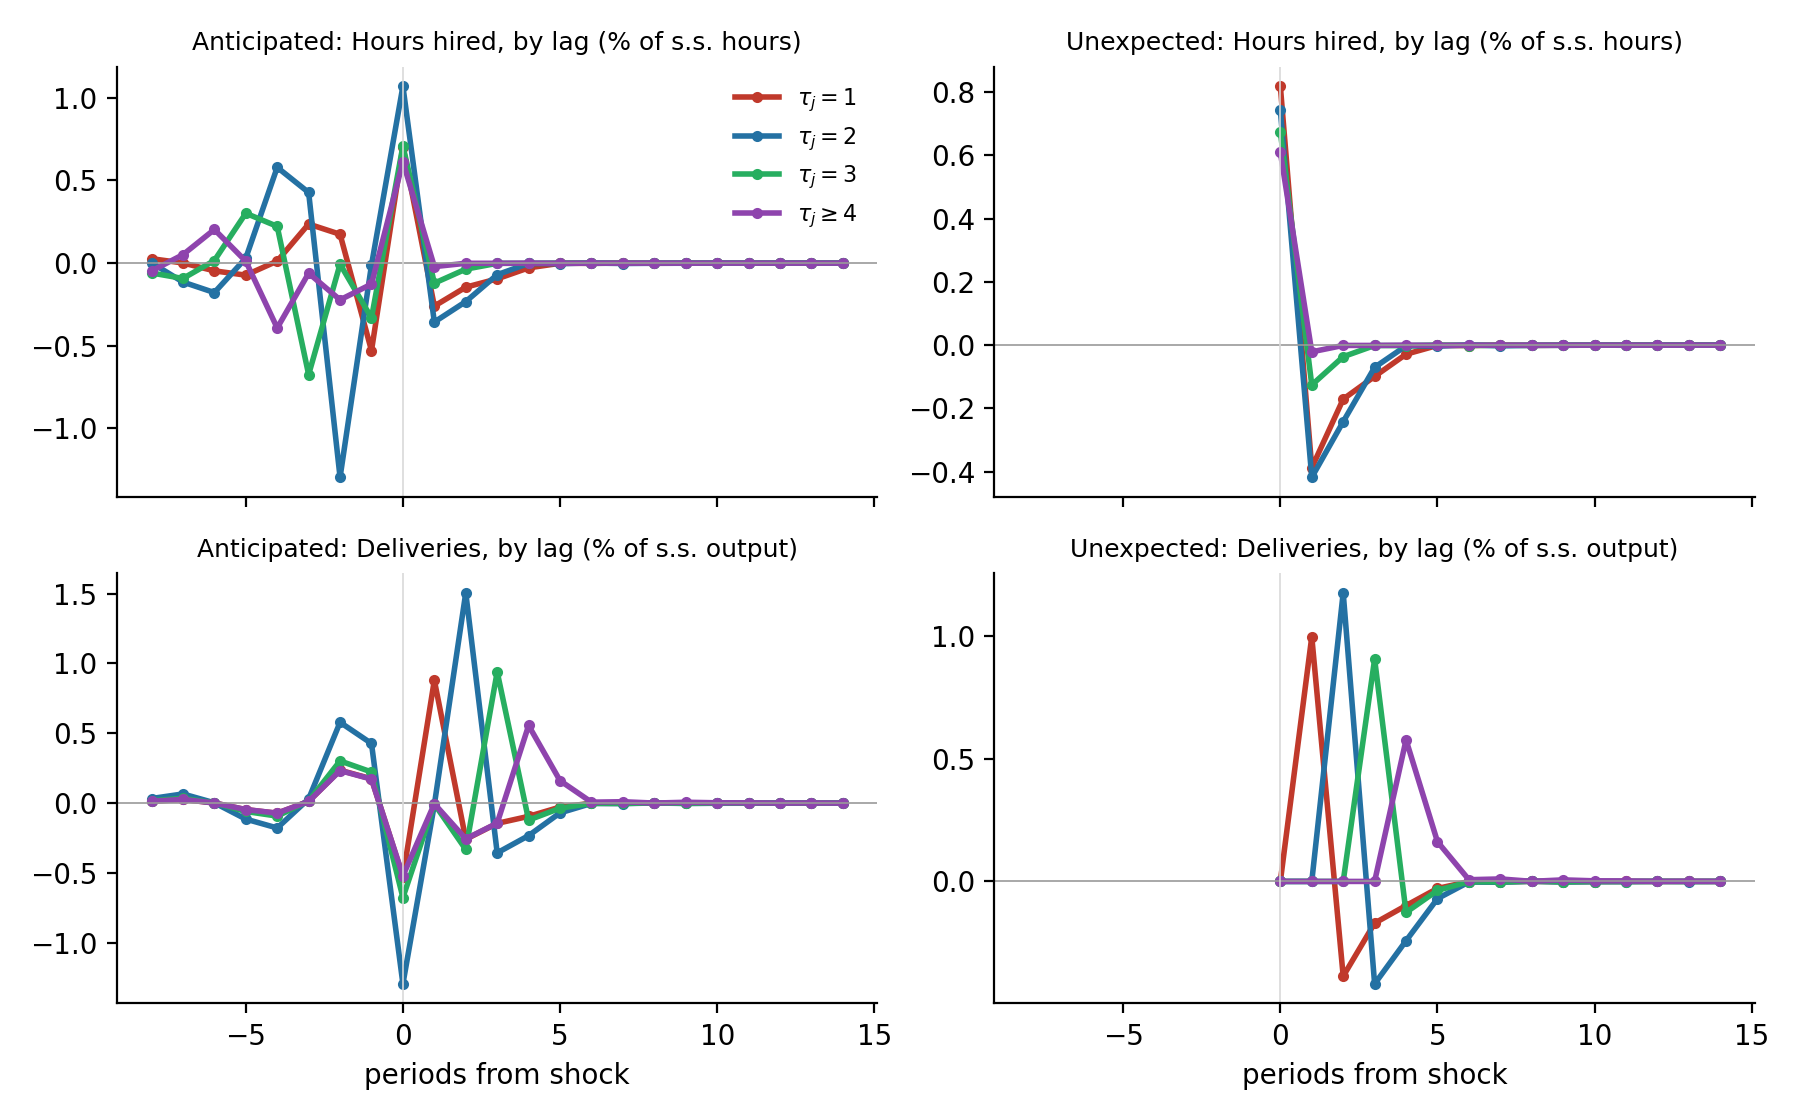
\includegraphics[width=\textwidth]{ce_tfp_bylag.png}
  \caption{The productivity shock by lag group. Top: hours hired at each date, by the lag of the
  producer (in \% of steady-state hours). Bottom: deliveries at each date, valued at steady-state
  prices (in \% of steady-state output).}
  \label{fig:ce_tfp_bylag}
\end{figure}

\subsection{An interest-rate shock}

Figure~\ref{fig:ce_rate} shows a one-month rise in the interest rate of 1 percentage point
annualised (0.083 points a month) at date 0.

\paragraph{No time to build.} Nothing happens. The rate enters costs only over the production
window, and there is none (Corollary~\ref{cor:first}(d)).

\paragraph{Unexpected.} The rise makes every batch whose production window spans date 0 more
expensive, so hiring falls by 0.30\% at date 0. Goods sold at date 0 are committed, so the price level
has to rise, by 0.56\%, for the household to accept fewer hours at the same consumption. Profits rise
by 0.87\% of steady-state output. From date 1 the costlier batches are delivered. The price level stays
above steady state for four months, the real wage is lower, and output falls by 0.08\%, 0.06\% and
0.03\%. Cumulative output falls by 0.16\%.

\paragraph{Anticipated.} The rate rise is a cost shock to the batches started in the $\tau_j$ periods
before it. The price level rises by $\bar S_k\iota$ at horizon $k\ge1$, about 0.08\%, 0.07\% and 0.03\%
over the first three months. Hiring falls on the shock date, and with an unchanged real wage,
consumption rises by 0.22\%. Before the shock, hours and consumption again move in opposite
directions. Cumulative output falls by 0.05\%, as \eqref{eq:cum} predicts.

\begin{figure}[h]
  \centering
  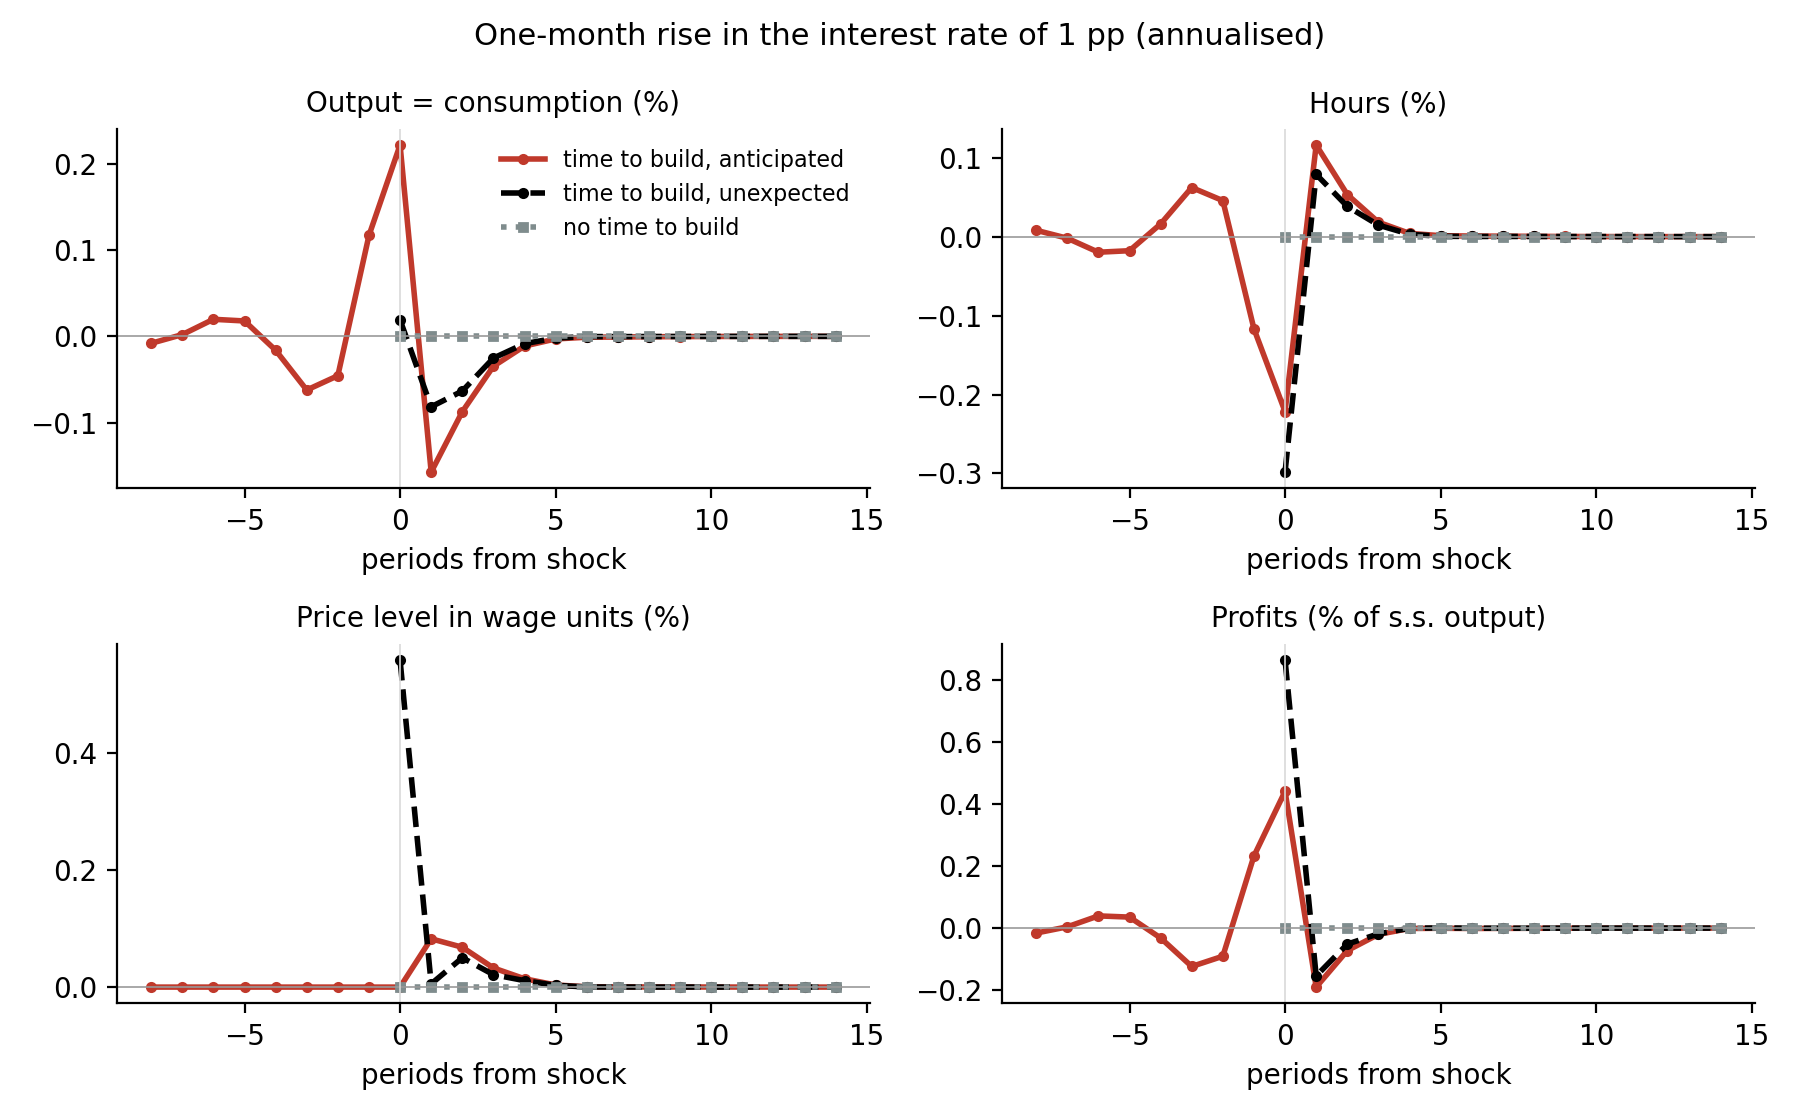
\includegraphics[width=\textwidth]{ce_rate.png}
  \caption{A one-month rise in the interest rate of 1 percentage point annualised at date 0.
  Competitive economy with fixed durations.}
  \label{fig:ce_rate}
\end{figure}

\begin{table}[h]
  \centering
  \caption{Propagation in the competitive economy (\% deviations from steady state; profits in \% of steady-state output; TTB = time to build)}\label{tab:prop}
  \small\setlength{\tabcolsep}{4pt}
  \begin{tabular}{lcccccc}
    \toprule
    & \multicolumn{3}{c}{1\% productivity} & \multicolumn{3}{c}{1 pp (annualised) interest rate} \\
    \cmidrule(lr){2-4}\cmidrule(lr){5-7}
    & no TTB & unexpected & anticipated & no TTB & unexpected & anticipated \\
    \midrule
    Output, date 0           & 0.75 & $-0.13$ & $-3.05$ & 0 & 0.02 & 0.22 \\
    Output, dates 1--4        & 0    & 2.17    & 1.88    & 0 & $-0.18$ & $-0.29$ \\
    Output, before date 0     & 0    & 0       & 1.90    & 0 & 0 & 0.02 \\
    Cumulative output         & 0.75 & 2.08    & 0.76    & 0 & $-0.16$ & $-0.05$ \\
    Cumulative hours          & $-0.25$ & 1.03 & $-0.25$ & 0 & $-0.16$ & $-0.05$ \\
    Hours, date 0             & $-0.25$ & 2.68 & 3.05    & 0 & $-0.30$ & $-0.22$ \\
    Price level, date 0       & $-1.00$ & $-5.11$ & $-0.01$ & 0 & 0.56 & 0 \\
    Profits, date 0           & 0 & $-8.16$ & $-6.09$ & 0 & 0.87 & 0.44 \\
    \midrule
    Cumulative output, linear & 0.75 & -- & 0.75 & 0 & -- & $-0.05$ \\
    \bottomrule
  \end{tabular}
\end{table}

\subsection{How small is ``small''?}\label{sec:howsmall}

The responses above hold durations fixed. Proposition~\ref{prop:local} justifies this for shocks
smaller than the gap $g$, and in the calibration that gap is tiny. Near its maximum $z_j(\cdot)$ is
flat, so the loss from producing one period longer or shorter is second order. Across producers,
the gap $1-\max_{\Delta\neq\tau_j}z_j(\Delta)/z_j(\tau_j)$ has a median of 0.11\% and a maximum of
0.22\%. It is close to zero for producers whose data duration is near a half-integer.

To check the fixed-duration responses, we compute the value of every alternative duration along the
equilibrium path. A producer wants to change its duration if some alternative is worth more than the
wage. Measured by expenditure share:
\begin{itemize}
  \item for a productivity shock of 0.01\%, 2\% of producers would change their duration;
  \item at 0.1\%, 47\%;
  \item at 0.3\% or more, all of them.
\end{itemize}
For the rate shock, the share is 17\% when the shock is anticipated and 32\% when it is unexpected. The profitable changes re-time the batches started next to the shock. After a productivity
rise, the productive batch started at date 0 would rather be sold one or two months later or earlier, at a
date when the price of its good is set by less productive batches. After a rate rise, batches started
at date 1 would rather finish one month sooner, and be sold at the price set by the costlier batches
that spanned the rise.

The responses in this section, and the policy analysis that follows, should therefore be read as
those of an economy with fixed production lags $\tau_j$. With endogenous durations, re-timing
would spread each shock over more delivery dates.

% =====================================================================
\section{Optimal monetary policy}\label{sec:policy}

The economy of Section~\ref{sec:model} has no money and no saving: the interest rate is a cost of
carrying goods in production, and nobody chooses it. To study monetary policy we change two
things. The household can now save in nominal bonds, which brings in an Euler equation, and the
nominal wage is rigid. A central bank sets the nominal rate and chooses its path to maximise
household welfare. Producers and the final-good firm are unchanged. Prices are now in units of
currency, and producers discount at the nominal rate $i_t$.

% ---------------------------------------------------------------------
\subsection{The household with bonds}\label{sec:hhbonds}

The household has a preference shifter $\theta_t>0$, which we use as a demand shock. It chooses
consumption $C_t$, labour $L_t$ and one-period nominal bonds $B^h_t$ to solve
\begin{equation}\label{eq:hhb}
  \max_{\{C_t,L_t,B^h_t\}}\;\sum_{t=0}^{\infty}\beta^t\theta_t
     \Bigl(\frac{C_t^{1-\sigma}}{1-\sigma}-\chi\frac{L_t^{1+\eta}}{1+\eta}\Bigr)
  \quad\text{s.t.}\quad
  P_tC_t+B^h_t=W_tL_t+(1+i_{t-1})B^h_{t-1}+\Pi_t ,
\end{equation}
with $B^h_{-1}=0$. Bonds are in zero net supply, so $B^h_t=0$ in equilibrium and the budget
constraint reduces to that of Section~\ref{sec:model}. Bonds are never held, but their price
matters: the Euler equation
\begin{equation}\label{eq:euler}
  \theta_t\frac{C_t^{-\sigma}}{P_t}=\beta(1+i_t)\,\theta_{t+1}\frac{C_{t+1}^{-\sigma}}{P_{t+1}}
\end{equation}
ties the path of consumption to the nominal rate and inflation. With a flexible wage the household
is also on its labour-supply curve, $\chi L_t^{\eta}C_t^{\sigma}=W_t/P_t$. The demand shock $\theta_t$
enters only through \eqref{eq:euler}: it scales all of period-$t$ utility.

\paragraph{Neutrality with a flexible wage.} With a nominal wage $W_t$, zero profit gives the
nominal price of good $j$ delivered at $t$:
\begin{equation}\label{eq:nomprice}
  p_{j,t}=\frac{W_{t-\tau_j}\prod_{s=t-\tau_j}^{t-1}(1+i_s)}{\zeta_{j,t-\tau_j}\,A_{t-\tau_j}} .
\end{equation}
This is the wage paid at hiring, carried forward at the nominal rate over the production window,
per unit of output. Producers discount at the nominal rate, $\delta_s=1/(1+i_s)$, so a change in
the nominal rate changes both their discount factors and the prices in \eqref{eq:nomprice}. By
\eqref{eq:value} and \eqref{eq:nomprice}, the value of a worker hired at $t$ and sent to completion
date $\tau$, relative to the wage, is
\begin{equation}\label{eq:valnom}
  \frac{v_{j,t}(\tau)}{W_t}
  =\frac{W_{\tau-\tau_j}}{W_t}\,
   \frac{\prod_{s=\tau-\tau_j}^{\tau-1}(1+i_s)}{\prod_{s=t}^{\tau-1}(1+i_s)}\,
   \frac{\kappa^{\tau-t}(\tau-t+B_tN_j)A_t}{\zeta_{j,\tau-\tau_j}A_{\tau-\tau_j}} .
\end{equation}
Nominal rates enter only together with nominal wage growth, through $W_{s+1}/\bigl(W_s(1+i_s)\bigr)$:
wage growth net of the nominal rate. With a flexible wage, a change in the nominal rate changes
nominal wage growth one for one. This ratio, and hence every producer's choice, is unchanged.

\begin{proposition}[Neutrality with a flexible wage]\label{prop:neutral}
In the economy with household bonds and a flexible wage, with fixed durations, the equilibrium
allocation and relative prices are the same for every nominal-rate path that converges to the
steady state. Changing the path from $\{i_t\}$ to $\{i'_t\}$ multiplies the wage and every price at
date $t$ by $\prod_{s\ge t}(1+i_s)/(1+i'_s)$, so the nominal rate determines only inflation.
\end{proposition}

\noindent The proof is in Appendix~\ref{app:pf_neutral}. Comparing with Section~\ref{sec:model}, the interest rate
has real effects there only because the household cannot save, so nothing ties the rate at which
producers discount to the household's real rate. Once the household can save, time to build alone does not give monetary
policy real effects. A nominal rigidity is needed, and we use a rigid wage.

% ---------------------------------------------------------------------
\subsection{Rigid wage}\label{sec:rigid}

The nominal wage is fixed at its steady-state level, $W_t=\bar W$ for all $t$, and we normalise
$\bar W=1$. The household supplies the hours producers demand at that wage. It is therefore off its
labour-supply curve, and its problem becomes
\begin{equation}\label{eq:hhrigid}
  \max_{\{C_t,B^h_t\}}\;\sum_{t=0}^{\infty}\beta^t\theta_t
     \Bigl(\frac{C_t^{1-\sigma}}{1-\sigma}-\chi\frac{L_t^{1+\eta}}{1+\eta}\Bigr)
  \quad\text{s.t.}\quad
  P_tC_t+B^h_t=\bar WL_t+(1+i_{t-1})B^h_{t-1}+\Pi_t ,
\end{equation}
with $L_t$ taken as given. The only first-order condition is the Euler equation \eqref{eq:euler}. The gap
between the real wage and the marginal rate of substitution,
\begin{equation}\label{eq:wedge}
  \mathcal W_t\equiv\log\frac{\bar W}{P_t}-\log\bigl(\chi L_t^{\eta}C_t^{\sigma}\bigr),
\end{equation}
is zero in the steady state and measures the friction away from it. When $\mathcal W_t>0$ the
household works less than it would like at the going real wage.

With $W_t=\bar W$, prices in currency coincide with prices in units of labour. The producer side is
therefore exactly that of Section~\ref{sec:model}: zero profit gives \eqref{eq:price}, with goods from
batches started before date 0 priced by demand.

\begin{definition}[Equilibrium with a rigid wage]\label{def:eqrigid}
Given initial conditions, a nominal-rate path $\{i_t\}_{t\ge0}$ and shocks $\{A_t,B_t,\theta_t\}_{t\ge0}$,
an equilibrium with a rigid wage consists of prices $\{P_t,\{p_{j,t}\}_j\}$ and allocations as in
Definition~\ref{def:eq} such that: the household solves \eqref{eq:hhrigid}; the final-good firm and
producers optimise as in Section~\ref{sec:model} with $W_t=\bar W$; $C_t=Y_t$, $L_t=\sum_jl_{j,t}$ and
$B^h_t=0$; and $(C_t,L_t,P_t)\to(C,L,P)$.
\end{definition}

\paragraph{Fixed durations.} In the policy analysis we hold each producer's duration at its
steady-state value, $\tau_{j,t}=t+\tau_j$. There are three reasons.
\begin{itemize}
  \item \emph{Tractability.} With endogenous durations, each producer can split a batch across
        several completion dates. The equilibrium is then a complementarity problem at every date,
        and the planner would have to optimise over it. With fixed durations, the planner's
        constraint set is a system of smooth equations.
  \item \emph{Local justification.} By Proposition~\ref{prop:local}, fixed durations are an
        equilibrium for small enough shocks.
  \item \emph{Timescales.} Durations respond to permanent changes in growth and the interest rate
        (Proposition~\ref{prop:growth}). We read them as a feature of technology that adjusts slowly,
        not as a margin firms re-optimise in response to a one-period shock.
\end{itemize}
The cost is that, in the calibration, the region where fixed durations are an equilibrium is
small (Section~\ref{sec:howsmall}). Policy with endogenous durations is left for future work.

\noindent With fixed durations the equilibrium has a simple recursive structure.
\begin{enumerate}
  \item \emph{Prices are set by costs.} For $t\ge\max_j\tau_j$, $P_t$ follows from \eqref{eq:price}
        given past rates and productivity. Before that, the price of committed goods also depends on
        $Y_t$. The fixed wage anchors the price level, so it is determinate without a further
        condition.
  \item \emph{Consumption is set by the Euler equation.} Given $\{P_t\}$, \eqref{eq:euler} and
        $C_t\to C$ determine $\{C_t\}$ backwards from the terminal date.
  \item \emph{Hours are set by demand.} Producers hire $l_{j,t}=\tilde y_{j,t+\tau_j}/(\zeta_jA_t)$ to
        deliver the demanded quantities, and $L_t=\sum_jl_{j,t}$.
\end{enumerate}
The nominal rate now moves the real rate, through two channels. As in any New Keynesian model, it
enters the Euler equation and shifts consumption over time. With time to build, it also enters
producers' costs over the production window, as in Section~\ref{sec:model}, which moves prices and
inflation for $\max_j\tau_j$ periods. Without time to build ($\tau_j=0$), $P_t=\bar W/\tilde A_t$
depends only on current productivity, and only the first channel is active.

% ---------------------------------------------------------------------
\subsection{The planner's problem}\label{sec:ramsey}

The central bank chooses the nominal-rate path to maximise household welfare, taking as constraints
the equilibrium conditions with a rigid wage. It commits to the whole path at the first date it acts,
$t_p$:
\begin{equation}\label{eq:ramsey}
  \max_{\{i_t\}_{t\ge t_p}}\;\sum_{t\ge t_p}\beta^{t-t_p}\theta_t
     \Bigl(\frac{C_t^{1-\sigma}}{1-\sigma}-\chi\frac{L_t^{1+\eta}}{1+\eta}\Bigr)
\end{equation}
subject to
\begin{enumerate}
  \item $\{C_t,L_t,P_t,\dots\}$ is an equilibrium with a rigid wage given $\{i_t\}$, the shocks, and the
        information private agents have (Section~\ref{sec:info_struct});
  \item $0\le i_t\le\bar\imath$, a zero lower bound and an upper bound that never binds at the optimum;
  \item $i_t=\rho\equiv1/\beta-1$ for $t\ge t_p+H$: after $H$ free months the rate returns to the peg.
\end{enumerate}
The planner does not choose allocations directly. It chooses rates, and allocations follow from
the private equilibrium.

\paragraph{Benchmarks.} The \emph{peg} keeps $i_t=\rho$ throughout. The \emph{flexible-wage}
allocation is the equilibrium with $W_t$ free and the household on its labour-supply curve. By
Proposition~\ref{prop:neutral} it does not depend on policy, and we use it as a reference.

\paragraph{The steady state.} With $\bar W$ at its steady-state level, the wedge
\eqref{eq:wedge} is zero, producers discount at $\delta=\beta$, and goods are priced at marginal cost.
Without shocks, the peg is optimal: no permanent deviation of the rate from $\rho$ raises welfare. With
a markup ($p_{j,t}=\mu\times$ marginal cost with $\mu>1$) the steady state would be inefficient, and the
planner would use the rate to push output above it: an inflation-bias problem. We keep $\mu=1$
throughout and return to commitment in Section~\ref{sec:concl}.

% ---------------------------------------------------------------------
\subsection{Shocks and information}\label{sec:info_struct}

We consider two shocks, each lasting one month at date 0:
\begin{itemize}
  \item a 3\% fall in productivity, $A_0=0.97$, which hits the batches started at date 0;
  \item a 1\% fall in demand, $\theta_0=e^{-0.01}$.
\end{itemize}
They differ in timing. The productivity shock hits production when it starts, so it reaches output
at each producer's delivery date. The demand shock hits the household at date 0, when almost all
goods on sale come from committed batches.

The information structures are as follows.
\begin{itemize}
  \item \emph{Unexpected.} Everyone learns of the shock at date 0, and batches started before date 0
        are committed. The planner acts from $t_p=0$.
  \item \emph{Expected, horizon $k$.} Everyone learns of the shock at date $-k$, and batches started
        after $-k$ are planned with the shock in mind. We consider the planner acting from the news
        date, $t_p=-k$, and acting only from the shock date, $t_p=0$. At $k=\max_j\tau_j=13$ no batch
        is committed when the shock hits.
  \item \emph{Planner informed.} The planner learns of the shock at $-k$ and commits to a rate path.
        Private agents observe the path but believe there is no shock until date 0. At date 0 everyone
        learns, and deliveries already in production stay at the quantities planned under the old
        beliefs.
\end{itemize}

\paragraph{Welfare.} We report the gain from optimal policy over the peg,
$100\,(U^{opt}-U^{peg})/C^{1-\sigma}$, in per cent of one month's steady-state consumption. We split
it into a consumption term and an hours term, following the two parts of period utility. To compare
horizons, all gains are valued at date $-13$, that is, discounted by $\beta^{13-k}$ from the news
date. Appendix~\ref{app:comp} describes the numerical method: the exact nonlinear model under perfect foresight,
with $H=8$ free months ($k+8$ when the planner acts from the news date).

% =====================================================================
\section{Optimal policy with and without time to build}\label{sec:results}

This section solves the planner's problem of Section~\ref{sec:policy} for each shock and information
structure, and compares the result with the same economy without time to build: $\tau_j=0$ for all
$j$, with the same $\zeta_j$, wage rigidity and preferences. Table~\ref{tab:policy} summarises
the comparison, and Table~\ref{tab:horizon} reports the welfare gains by news horizon. In every
figure, red is time to build and black is no time to build; solid lines are the optimal rate and
dotted lines the peg. Rates are annualised; the steady-state rate is 4\%. Gains are in per cent of
one month's steady-state consumption, valued at $t=-13$, and TTB abbreviates time to build in the
tables.

Four differences run through the results.
\begin{enumerate}
  \item \emph{The optimal rate moves the other way.} Without time to build the rate works only
        through the Euler equation. With time to build it is also a cost of production, so the planner
        cuts it to support hiring after a productivity fall, where the standard model hikes.
  \item \emph{Policy acts over more months and earlier.} Production commitments last up to
        $\max_j\tau_j$ months, so the planner spreads its response over several months after the
        shock and, with news, starts moving almost a year before it.
  \item \emph{The zero lower bound binds for different shocks.} With time to build the bound binds
        after supply shocks, because the optimal response is a cut. Without time to build it binds
        after demand shocks, as in the standard model.
  \item \emph{Policy matters more for supply shocks and less for demand shocks.} Time to build makes
        a productivity shock more than thirty times as costly under the peg. It raises the gain from
        optimal policy by a factor of 10 to 50, even though the zero bound stops the planner from
        removing most of the loss. It shrinks both the cost of a demand shock and the gain from policy,
        because committed production absorbs the shock.
\end{enumerate}

\begin{table}[t]
  \centering
  \caption{Optimal policy with and without time to build}\label{tab:policy}
  \small\setlength{\tabcolsep}{3.5pt}
  \begin{tabular}{lcccc}
    \toprule
    & \multicolumn{2}{c}{3\% productivity fall} & \multicolumn{2}{c}{1\% demand fall} \\
    \cmidrule(lr){2-3}\cmidrule(lr){4-5}
    & TTB & no TTB & TTB & no TTB \\
    \midrule
    \multicolumn{5}{l}{\emph{A. Unexpected}}\\
    Optimal rate at $t=0$ (\% a year)        & 0.0 & 24.9 & 2.5 & 0.0 \\
    Months with $|i_t-\rho|>25$\,bp          & 7    & 1    & 2    & 2 \\
    Months at the zero lower bound           & 1    & 0    & 0    & 2 \\
    Loss of the peg vs.\ flexible wage        & 0.393 & 0.0114 & 0.0022 & 0.0047 \\
    Gain from optimal policy                 & 0.123 & 0.0114 & 0.0022 & 0.0036 \\
    \quad consumption term / hours term      & $+0.42/-0.30$ & $-0.74/+0.76$ & $+0.28/-0.28$ & $+0.48/-0.47$ \\
    Share of the peg's loss removed          & 31\% & 100\% & 100\% & 77\% \\
    \midrule
    \multicolumn{5}{l}{\emph{B. Announced 13 months ahead, policy from the news date}}\\
    First month with $|i_t-\rho|>25$\,bp     & $-11$ & $-3$ & $-5$ & $-1$ \\
    Optimal rate at $t=-1$ / $t=0$ (\% a year) & 25.4 / 0.0 & 0.0 / 15.0 & 4.9 / 2.6 & 12.6 / 0.0 \\
    Gain from optimal policy                 & 0.384 & 0.0077 & 0.0024 & 0.0036 \\
    \quad consumption term / hours term      & $-1.72/+2.10$ & $-0.75/+0.75$ & $+0.46/-0.46$ & $+0.48/-0.47$ \\
    Share of the peg's loss removed          & 54\% & 67\% & 100\% & 77\% \\
    \midrule
    \multicolumn{5}{l}{\emph{C. Announced 13 months ahead, policy only from the shock date}}\\
    Gain from optimal policy                 & 0.106 & 0.0008 & 0.0011 & 0.0003 \\
    Share of the peg's loss removed          & 15\% & 7\% & 46\% & 7\% \\
    \bottomrule
  \end{tabular}

  \medskip
  \parbox{0.95\textwidth}{\footnotesize Losses and gains in \% of one month's steady-state
  consumption, valued at $t=-13$. The consumption and hours terms split the gain into the two
  parts of period utility. ``Share removed'' is the gain divided by the peg's loss relative to the
  flexible-wage allocation. Rates are annualised.}
\end{table}

% ---------------------------------------------------------------------
\subsection{Unexpected shocks}\label{sec:unexp}

\paragraph{Productivity.} Figure~\ref{fig:unexp_tfp} shows a 3\% fall in productivity at date 0.

Without time to build, the shock raises unit costs at once. With the wage fixed, the price level jumps
by 3\% and output falls. The planner \emph{raises} the rate for one month, to 25\% annualised (1.9
points in the month). Lower productivity makes the efficient level of output lower, and the hike moves
consumption down to it and saves hours. Policy removes the whole loss of the peg.

With time to build, the shock hits the batches started at date 0, and the goods sold at date 0 come
from batches already committed. Under the peg, hiring collapses by 5.8\% at date 0, and output and
prices respond only when the affected batches are delivered, from month 1. The planner \emph{cuts}
the rate to zero. Through the cost channel, the cut lowers the cost of carrying the batches started
at date 0 and offsets part of the productivity loss. Hiring falls by 4.7\% instead of 5.8\%, output in
months 1--2 falls less, and inflation is spread out. The rate then rises above the peg, to 6\% in
month 2, and stays above it for several months.

The peg's loss is more than thirty times as large as without time to build, and the gain from optimal
policy is eleven times as large. Policy removes only 31\% of the loss, for two reasons:
\begin{itemize}
  \item nothing can be done about the batches committed before the shock;
  \item the zero lower bound stops the cut at 4 points.
\end{itemize}
The gain comes from consumption, at a cost in hours.

\paragraph{Demand.} Figure~\ref{fig:unexp_dem} shows a 1\% fall in demand. Without time to build,
this is the textbook case: the planner cuts the rate to zero. Here the bound binds for two months, and
policy removes 77\% of the loss.

With time to build, almost all goods sold at date 0 are committed. Output hardly moves ($-0.03\%$
under the peg), and the shock falls on prices instead ($-0.94\%$). The planner cuts the rate only to
2.5\%, which raises hiring for future deliveries and cushions the fall in prices. It removes the whole
loss, but the loss is half as large as without time to build.

\paragraph{The zero lower bound.} Time to build changes which shocks take the economy to the zero
bound. In the standard model the bound is a problem for demand shocks. With time to build it is not:
committed production absorbs the demand shock, and a small cut is enough. The bound instead binds for
supply shocks, because time to build turns the optimal response to a productivity fall from a hike
into a cut. The bound is also the main reason policy removes only a third of the loss from an
unexpected productivity shock.

\begin{figure}[t]
  \centering
  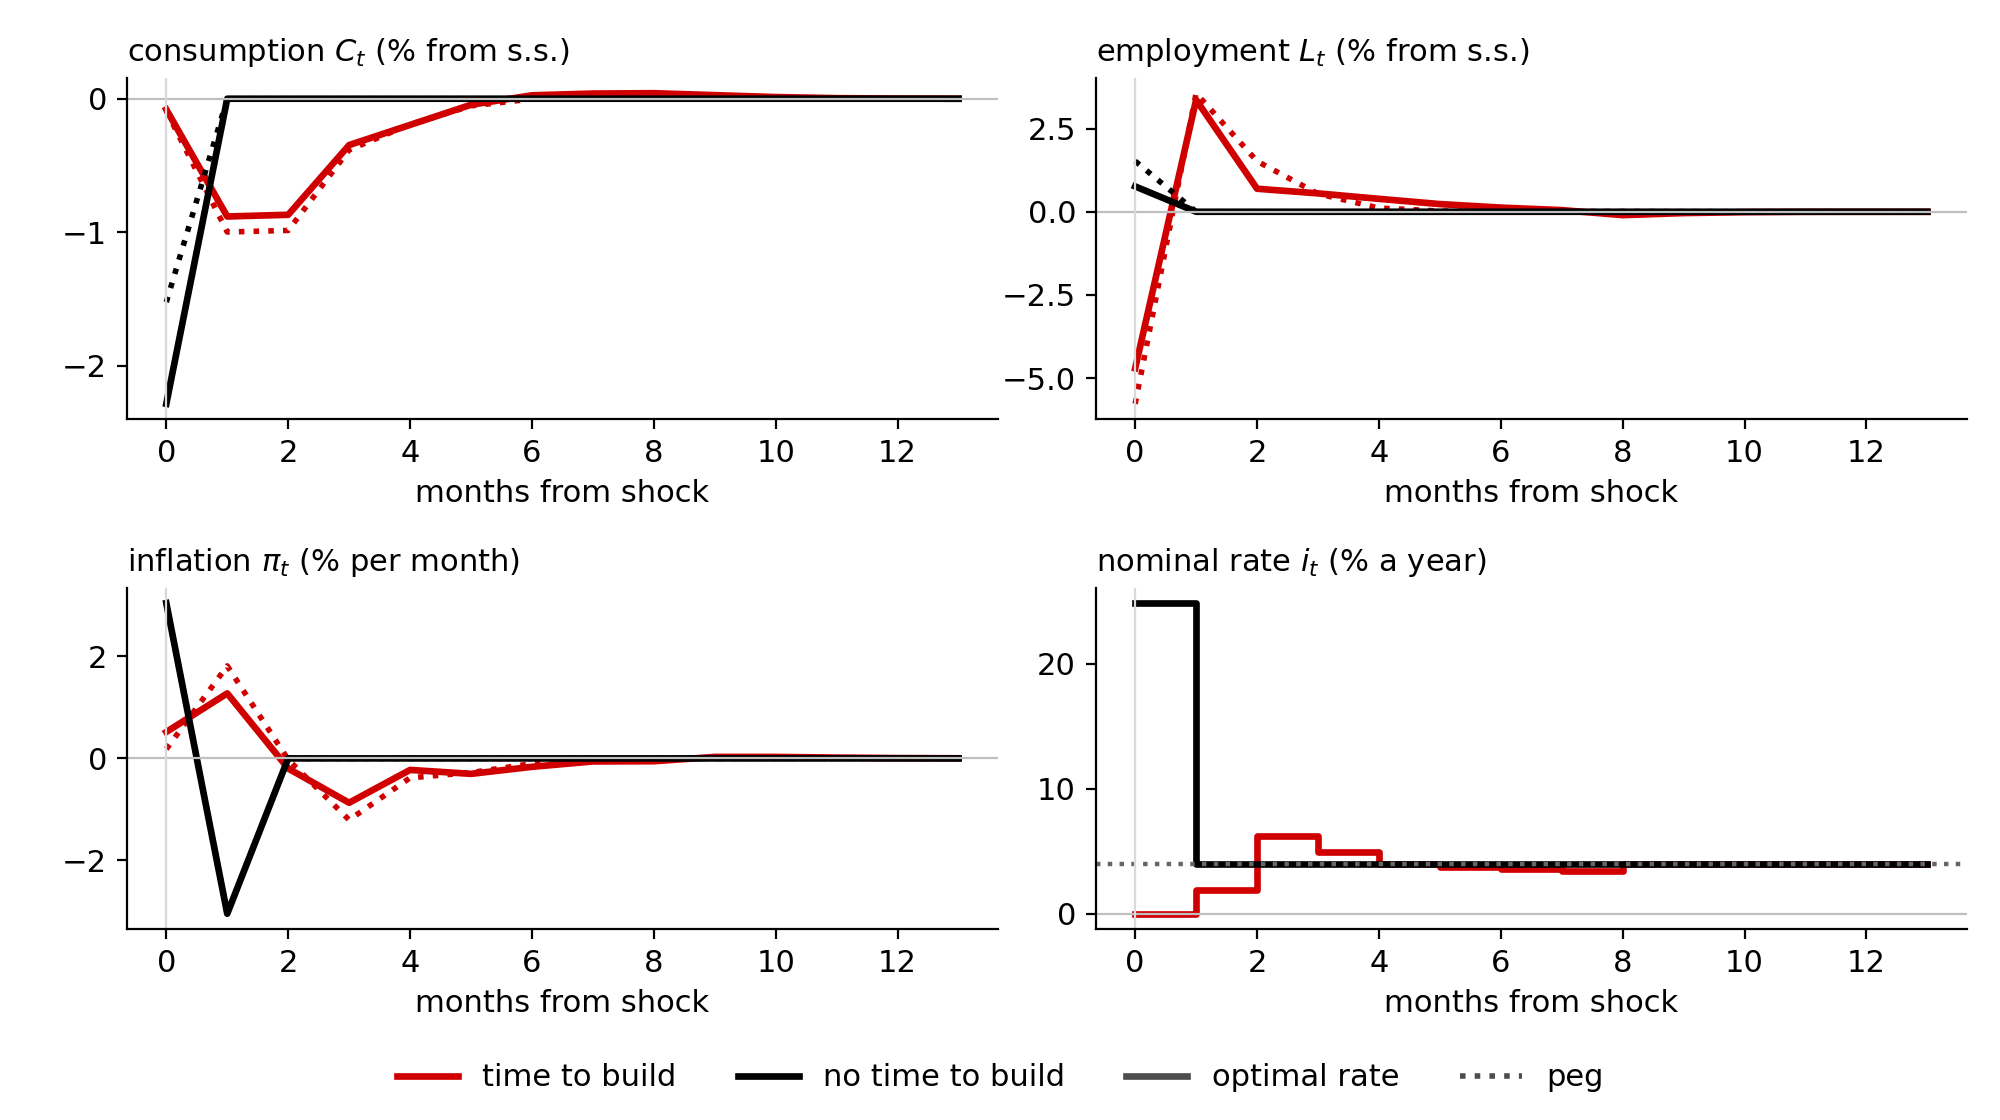
\includegraphics[width=\textwidth]{pol_unexp_tfp.png}
  \caption{Unexpected 3\% fall in productivity at $t=0$. Red: time to build; black: no time to
  build. Solid: optimal rate; dotted: peg. Rates annualised.}
  \label{fig:unexp_tfp}
\end{figure}

\begin{figure}[t]
  \centering
  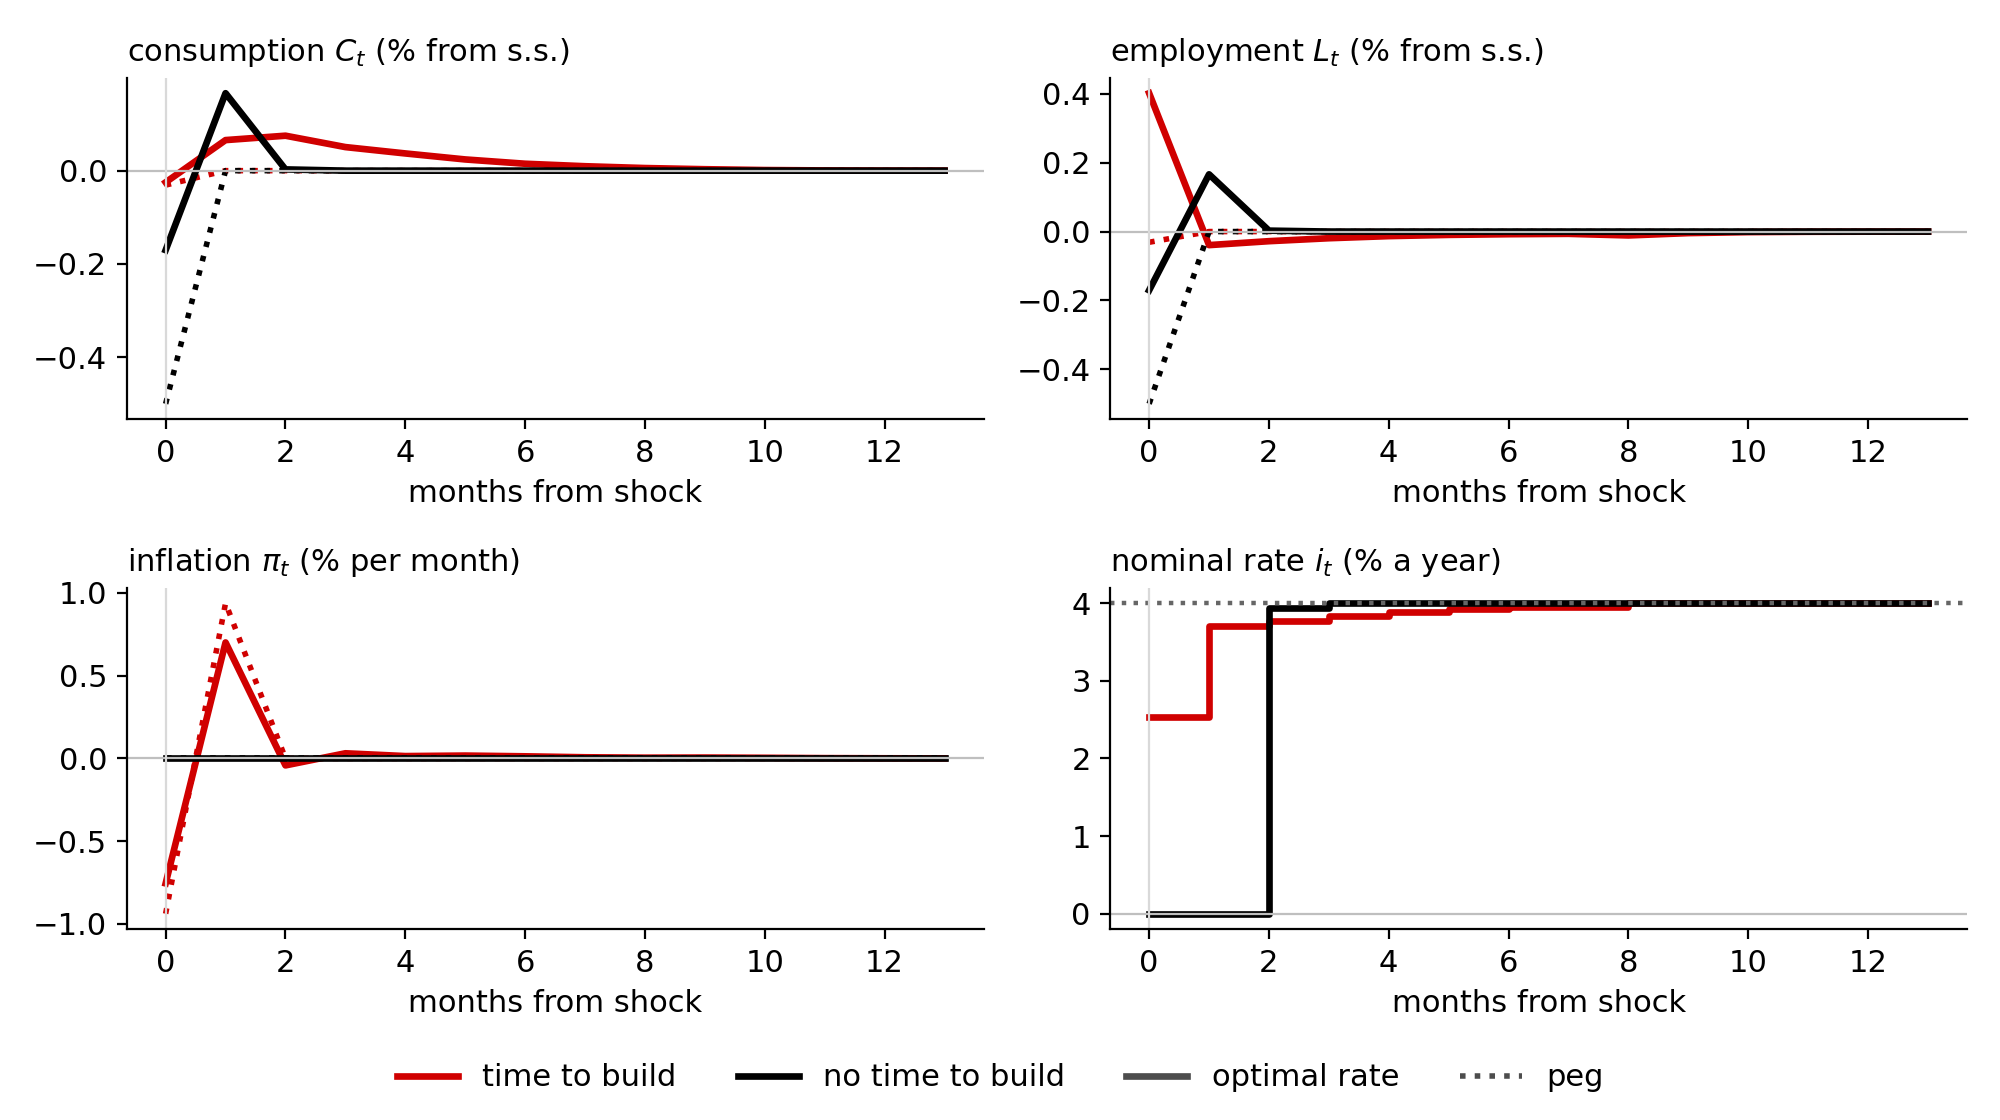
\includegraphics[width=\textwidth]{pol_unexp_dem.png}
  \caption{Unexpected 1\% fall in demand at $t=0$. Red: time to build; black: no time to build.
  Solid: optimal rate; dotted: peg. Rates annualised.}
  \label{fig:unexp_dem}
\end{figure}

% ---------------------------------------------------------------------
\subsection{Expected shocks}\label{sec:exp}

\paragraph{Policy from the news date.} Figure~\ref{fig:exp_tfp} shows the productivity shock announced
13 months ahead.

Without time to build, the planner leaves the rate at the peg until three months before the shock.
It lowers the rate to 1.7\% at $t=-3$, cuts it to zero for the two months before the shock, where the
bound binds, and raises it to 15\% at $t=0$.

With time to build, under the peg, firms bring hiring forward to produce before the shock: hours rise
by 2.7\% at $t=-1$ and then collapse by 8.5\% at $t=0$. The planner starts moving eleven months early,
lowering the rate gradually to about 2\%. It then raises it to 25\% at $t=-1$, which stops the hiring
rush, and cuts it to zero at $t=0$, which supports hiring when the shock hits. The timing is the reverse
of the case without time to build. The gain, 0.38, is three times the gain for an unexpected shock and
fifty times the gain without time to build. It comes from smoothing hours, at a cost in consumption.

For demand (Figure~\ref{fig:exp_dem}), the planner without time to build raises the rate to 12.6\% at
$t=-1$ and cuts it to zero at $t=0$. With time to build the rate stays within about one point of the
peg, rising slightly before the shock and falling to 2.6\% when it hits.

\paragraph{Policy only from the shock date.} If the planner cannot act before the shock, most of the
gain is lost in both economies (Table~\ref{tab:policy}, panel C). Without time to build, the rate at
$t=-1$ sets consumption at $t=-1$ relative to $t=0$ through the Euler equation, so a planner that acts
only from $t=0$ cannot undo the anticipation effect: it removes only 7\% of the loss. With time to
build, the hiring rush before the shock is out of the planner's reach. The gain, 0.11, is \emph{below}
the gain for an unexpected shock. Warning that the planner cannot use makes things worse: firms re-plan
for the shock, and the planner cannot steer how they do it.

\begin{figure}[t]
  \centering
  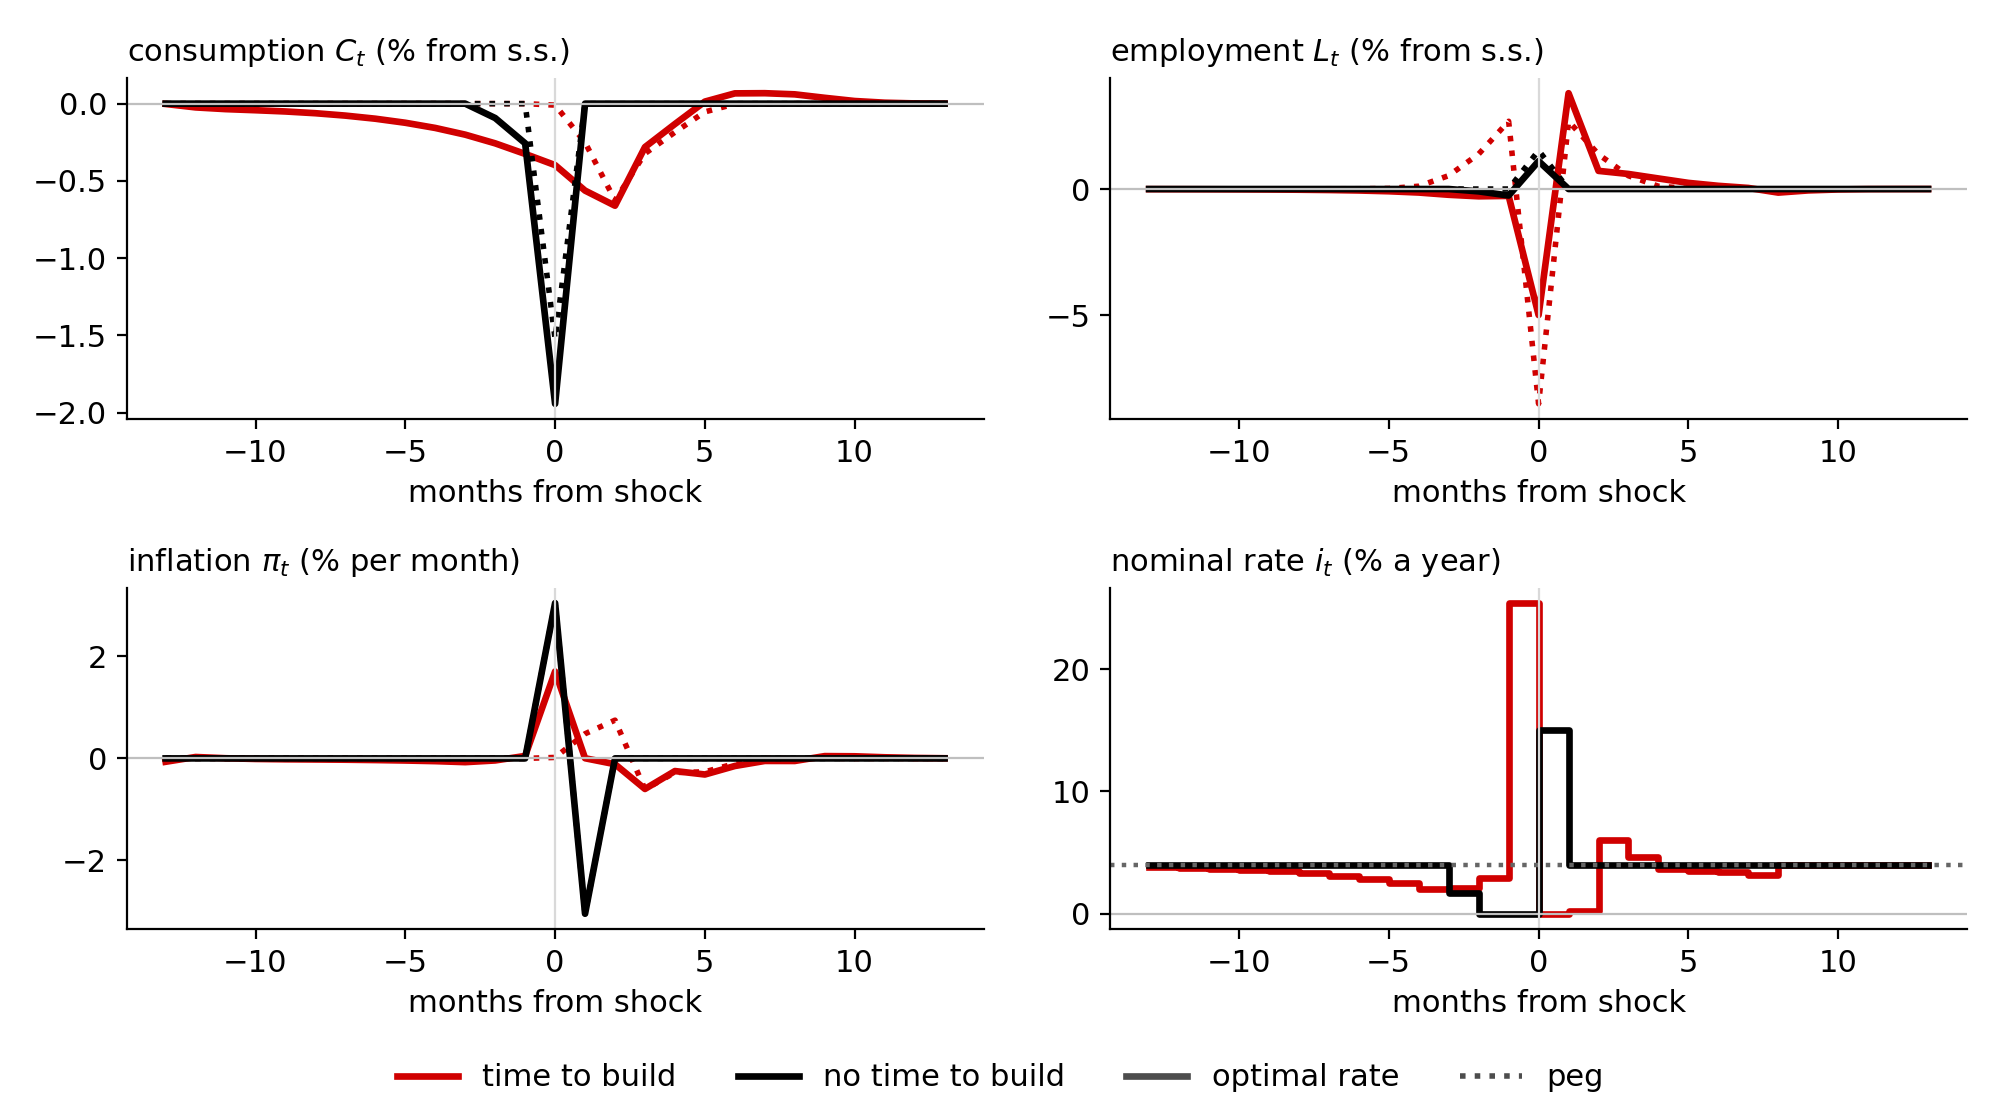
\includegraphics[width=\textwidth]{pol_exp_tfp.png}
  \caption{3\% fall in productivity announced 13 months ahead; policy free from the news date.
  Red: time to build; black: no time to build. Solid: optimal rate; dotted: peg. Rates annualised.}
  \label{fig:exp_tfp}
\end{figure}

\begin{figure}[t]
  \centering
  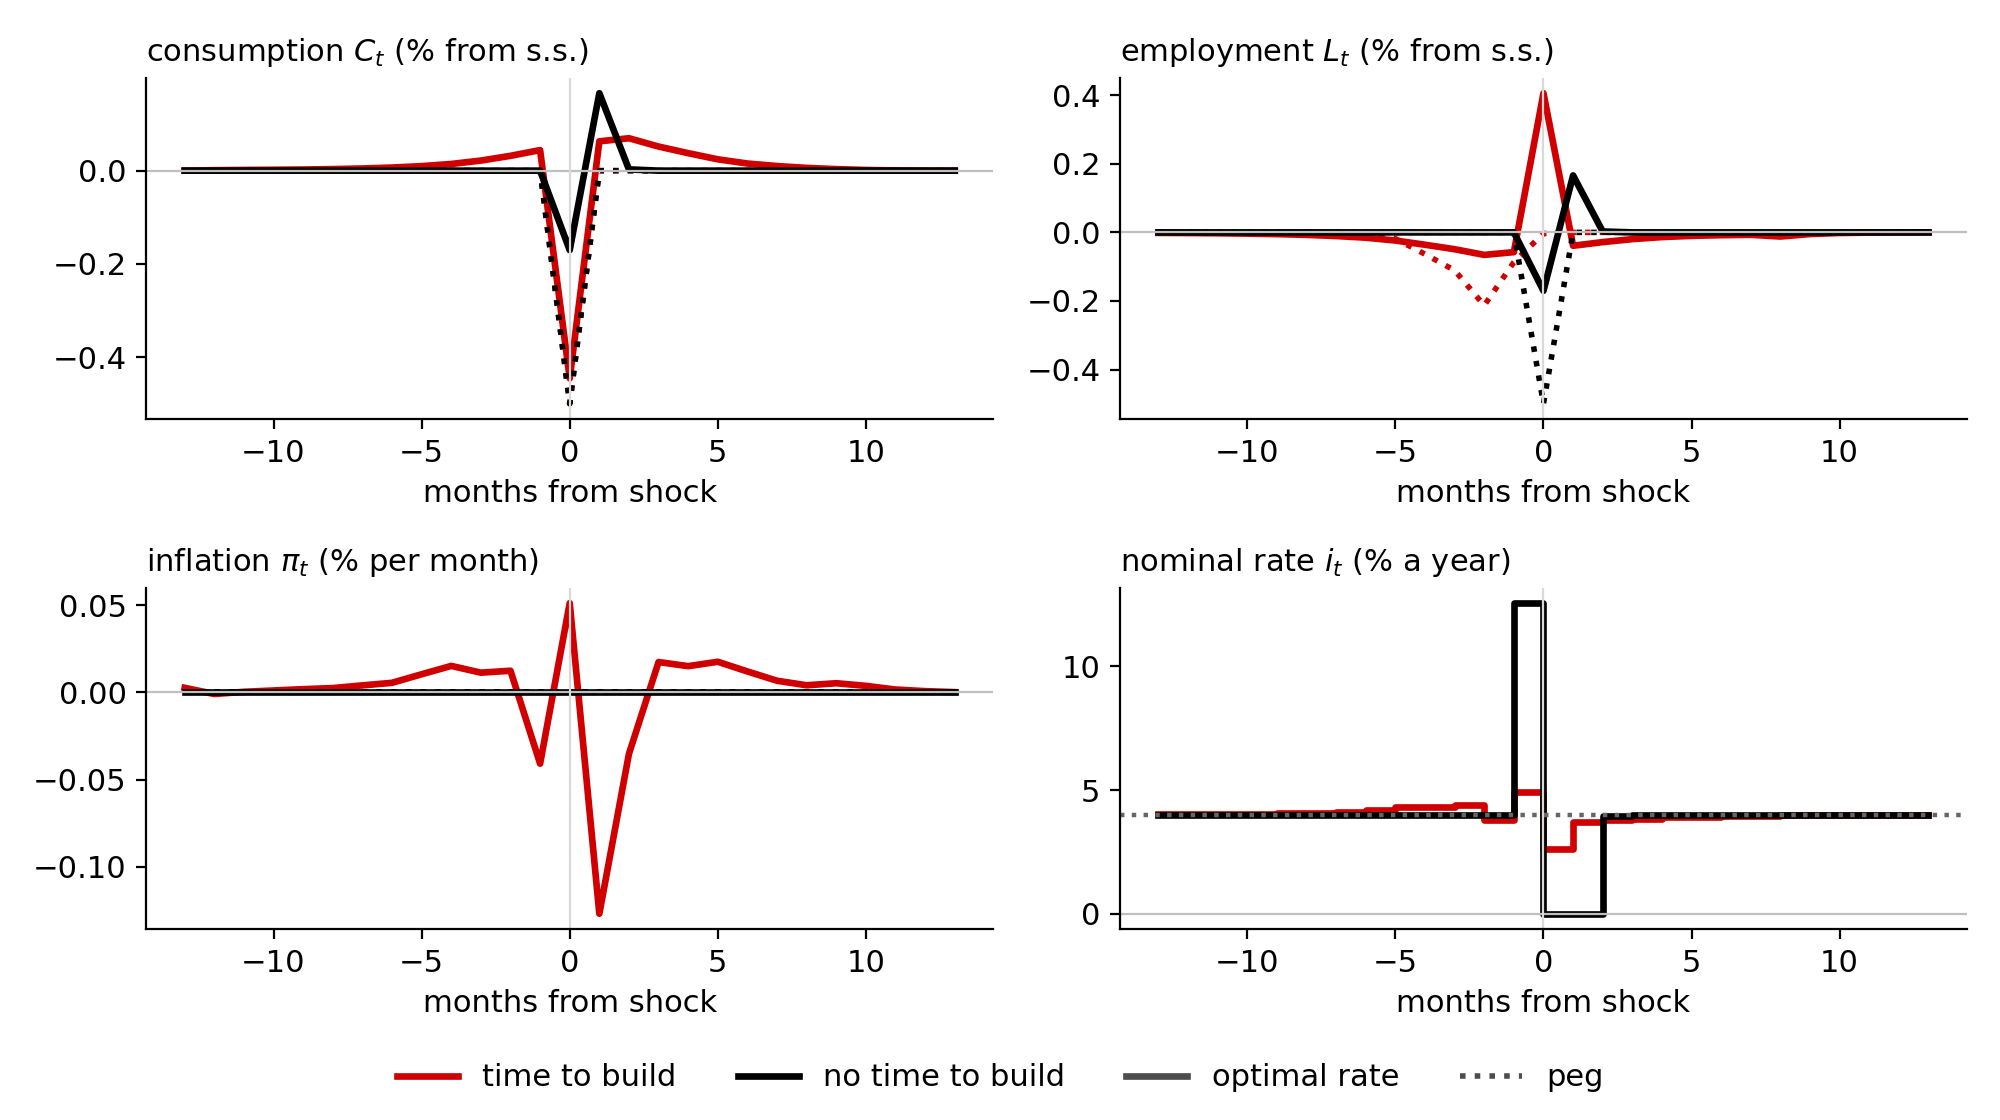
\includegraphics[width=\textwidth]{pol_exp_dem.png}
  \caption{1\% fall in demand announced 13 months ahead; policy free from the news date.}
  \label{fig:exp_dem}
\end{figure}

% ---------------------------------------------------------------------
\subsection{How much warning matters}\label{sec:warning}

Table~\ref{tab:horizon} and Figure~\ref{fig:horizon} vary the news horizon $k$, with policy free from
the news date.
\begin{itemize}
  \item \emph{Without time to build, warning does not help.} For demand the gain is the same at every
        horizon. For productivity it falls slightly with warning, from 0.0114 to 0.0077, because the
        planner hits the zero bound in the months before the shock.
  \item \emph{With time to build, one month of warning triples the gain from policy for a productivity
        shock}, from 0.12 to 0.37. A second month takes it to 0.39, and beyond that it is flat.
  \item \emph{For demand, short warning is worth most.} The gain is highest at $k=1$--2 ($2.7\times10^{-3}$)
        and settles at $2.4\times10^{-3}$. With a month or two of warning only the short-lag producers can
        re-plan, and policy can work through them.
\end{itemize}

\paragraph{Expectations or production commitment?} News does two things with time to build: it changes
expectations, and it lets firms re-plan production before the shock. To separate them, we solve a
\emph{commitment} case. News arrives at $-k$ and households and the planner react to it, but batches
started before date 0 stay at their steady-state quantities, as if the shock were unexpected. The
gain is then exactly the unexpected-shock gain at every horizon (Table~\ref{tab:horizon}). Better
information for the planner and households is worth nothing on its own. The whole value of warning
comes from firms re-planning production, which is why warning does not help without time to build.

\begin{table}[t]
  \centering
  \caption{Gain from optimal policy by news horizon $k$}\label{tab:horizon}
  \small\setlength{\tabcolsep}{5pt}
  \begin{tabular}{rcccccccc}
    \toprule
    & \multicolumn{4}{c}{3\% productivity fall} & \multicolumn{4}{c}{1\% demand fall ($\times10^{-3}$)} \\
    \cmidrule(lr){2-5}\cmidrule(lr){6-9}
    & \multicolumn{3}{c}{time to build} & no TTB & \multicolumn{3}{c}{time to build} & no TTB \\
    \cmidrule(lr){2-4}\cmidrule(lr){6-8}
    $k$ & everyone & commitment & planner only & everyone & everyone & commitment & planner only & everyone \\
    \midrule
    0  & 0.123 & 0.123 & 0.123 & 0.0114 & 2.18 & 2.18 & 2.18 & 3.65 \\
    1  & 0.371 & 0.123 & 0.129 & 0.0080 & 2.68 & 2.18 & 2.07 & 3.65 \\
    2  & 0.394 & 0.123 & 0.130 & 0.0077 & 2.71 & 2.18 & 2.14 & 3.65 \\
    3  & 0.392 & 0.123 & 0.131 & 0.0077 & 2.45 & 2.18 & 2.19 & 3.65 \\
    5  & 0.387 & 0.123 & 0.132 & 0.0077 & 2.34 & 2.18 & 2.23 & 3.65 \\
    13 & 0.384 & 0.123 & 0.131 & 0.0077 & 2.36 & 2.18 & 2.23 & 3.65 \\
    \bottomrule
  \end{tabular}

  \medskip
  \parbox{0.95\textwidth}{\footnotesize Gain $=$ optimal $-$ peg, \% of one month's steady-state
  consumption, valued at $t=-13$; policy free from the news date. \emph{Everyone}: all agents learn
  at $-k$. \emph{Commitment}: all agents learn at $-k$, but batches started before date 0 stay at
  their steady-state quantities. \emph{Planner only}: the planner learns at $-k$; firms and households
  learn at 0.}
\end{table}

\begin{figure}[t]
  \centering
  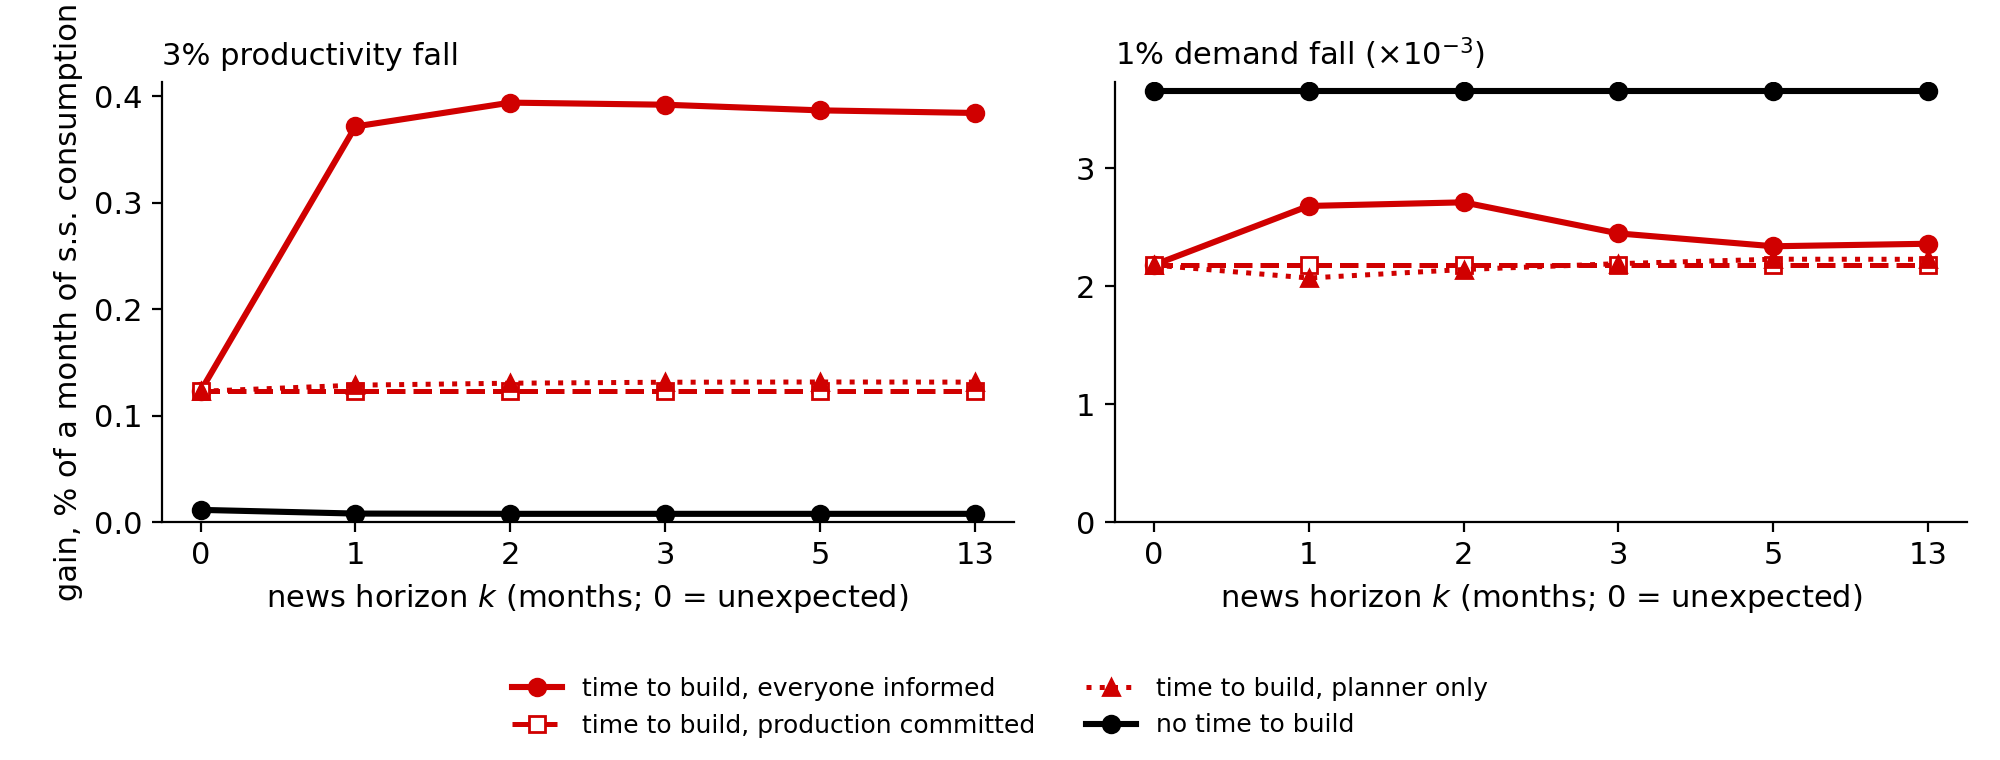
\includegraphics[width=\textwidth]{pol_horizon.png}
  \caption{Gain from optimal policy by news horizon $k$, valued at $t=-13$. Red: time to build
  (solid: everyone informed; dashed: production committed; dotted: planner only). Black: no time to
  build.}
  \label{fig:horizon}
\end{figure}

% ---------------------------------------------------------------------
\subsection{Who should know about the shock?}\label{sec:info}

Without time to build, warning does not help (Section~\ref{sec:warning}), so we study this question
with time to build only. There, warning matters through how firms re-plan. In the \emph{planner only}
case, the planner learns at $-k$ and commits to a path, and firms and households learn at date 0
(Section~\ref{sec:info_struct}).

\begin{itemize}
  \item \emph{Productivity.} The planner's own information is worth little: the gain rises only from
        0.123 to 0.131. But households are better off than when everyone is informed. Their utility
        relative to the no-shock steady state is $-3.128$ against $-3.188$ at $k=5$, and the advantage
        grows with the horizon. Public news of a cost shock triggers a hiring rush that the rigid wage
        cannot price, so it is better for firms not to know.
  \item \emph{Demand.} The ranking reverses: households are better off when everyone knows, by about
        $2\times10^{-3}$\% of a month's consumption, because public news lets production adjust to the
        fall in demand. At $k\le2$, the planner-only gain is even below the unexpected one. Firms build
        the announced rate moves into plans made for a world without the shock.
\end{itemize}

\clearpage
% =====================================================================
\section{Conclusion}\label{sec:concl}

Time to build changes how monetary policy should be conducted. When production takes time, the
interest rate is also the cost of carrying goods in production, and output responds to shocks at
each producer's delivery date rather than on impact. In a New Keynesian economy calibrated to industry
production lags, this reverses the optimal response to a productivity shock, from a hike to a cut. It
spreads policy over several months and makes policy far more valuable for supply shocks and less
valuable for demand shocks. Because the optimal response to a supply shock becomes a cut, the zero
lower bound binds after supply shocks rather than demand shocks. It also makes the timing of
information central. Warning about a shock is
worth something only because firms can re-plan production, and whether firms and households should
learn about a shock depends on whether it hits costs or demand.

\paragraph{Policy implications.} The interest rate should respond to where shocks fall in the
production pipeline, not only to their effect on current output and inflation. Rates should move
before an anticipated supply shock arrives, in the opposite direction to the move on arrival. Central
bank communication is part of the policy problem: announcing a cost shock early can make households
worse off by triggering a hiring rush, while announcing a demand shock early helps.

\paragraph{Commitment.} Every result assumes the planner commits at the first date it acts. Time to
build makes this assumption more consequential than usual. Before an anticipated shock, the optimal
path eases gradually and then raises the rate just before the shock, in order to shape how firms plan
production. Once those plans are made, a planner that re-optimised would want to change course, so
the path is unlikely to be time consistent. The incentive to deviate is stronger here than in the
standard model, for two reasons. Production committed before the shock is a fixed stock the planner can
exploit after the fact. And with a markup, an inefficient steady state adds the classic inflation
bias, which in our economy shows up as a boom in hiring. Solving for policy without commitment, and
measuring the value of commitment in each economy, is the natural next step. It would show whether
time to build widens the gap between rules and discretion.

\paragraph{Other extensions.} Four further directions are natural:
\begin{itemize}
  \item endogenous durations, so that policy affects when goods are delivered as well as how many are
        produced;
  \item wages that reset and shocks that persist;
  \item information design, in which announcements reveal what the planner knows;
  \item production networks, in which one producer's output is another's input and production
        lags compound along supply chains.
\end{itemize}

% =====================================================================
\bibliographystyle{plainnat}
% \bibliography{refs}

\clearpage
\appendix
\section{Proofs}\label{app:proofs}

Throughout, durations are bounded, $0\le\Delta\le T_j$, there are finitely many producers, and the
economy is in the steady state before date 0, so the initial conditions are
$y_{j,\tau|t}=y_{j}^{ss}$ for the batches started at $t<0$ and completed at $\tau=t+\tau_j\ge0$.
Write $\bar T\equiv\max_j\tau_j$.

% ---------------------------------------------------------------------
\subsection{The economy with fixed durations}\label{app:fixed}

When every producer uses its steady-state duration, $\tau_{j,s}=s+\tau_j$, only one vintage of each
good is delivered at each date, $\tilde y_{j,t}=y_{j,t|t-\tau_j}$, and the equilibrium conditions of
Definition~\ref{def:eq} reduce to the following, for all $t\ge0$ and $j$:
\begin{align}
  &\chi L_t^{\eta}C_t^{\sigma}=1/P_t, \tag{E1}\label{E1}\\
  &p_{j,t}/P_t=(Y_t/\tilde y_{j,t})^{1/\varepsilon},
  \qquad Y_t=\Bigl(\textstyle\sum_j\tilde y_{j,t}^{(\varepsilon-1)/\varepsilon}\Bigr)^{\varepsilon/(\varepsilon-1)}, \tag{E2}\label{E2}\\
  &p_{j,t}=\dfrac{\prod_{s=t-\tau_j}^{t-1}(1+i_s)}{\zeta_{j,t-\tau_j}A_{t-\tau_j}}\ \ (t\ge\tau_j),
  \qquad\tilde y_{j,t}=y_j^{ss}\ \ (t<\tau_j), \tag{E3}\label{E3}\\
  &l_{j,t}=\tilde y_{j,t+\tau_j}/(\zeta_{j,t}A_t),\qquad L_t=\textstyle\sum_jl_{j,t},
  \qquad C_t=Y_t, \tag{E4}\label{E4}
\end{align}
together with the terminal condition $(C_t,L_t)\to(C,L)$. Condition \eqref{E3} is zero profit
at the steady-state duration for batches started at or after date 0; deliveries from batches started
before date 0 are fixed by the initial conditions and priced by demand \eqref{E2}.

% ---------------------------------------------------------------------
\subsection{Mean lags}\label{app:meanlags}

By \eqref{eq:weights}, $\lambda_j\propto s_j\delta^{\tau_j}$, so
$\bar\tau_\lambda=\sum_js_j\tau_j\delta^{\tau_j}/\sum_js_j\delta^{\tau_j}$. The functions $\tau\mapsto\tau$
and $\tau\mapsto\delta^{\tau}$ are oppositely ordered when $\delta<1$. By Chebyshev's sum inequality,
$\sum_js_j\tau_j\delta^{\tau_j}\le\bigl(\sum_js_j\tau_j\bigr)\bigl(\sum_js_j\delta^{\tau_j}\bigr)$, with
equality only if $\tau_j$ is the same for all $j$ with $s_j>0$. Dividing by $\sum_js_j\delta^{\tau_j}$
gives $\bar\tau_\lambda\le\bar\tau_s$.\hfill$\blacksquare$

% ---------------------------------------------------------------------
\subsection{Proof of Proposition~\ref{prop:growth}}\label{app:pf_growth}

\emph{Step 1: prices on the path.} On a balanced growth path producer $j$ uses a constant duration
$\tau_j$, so by zero profit at that duration the price of good $j$ delivered at $t$ is
\[
  p_{j,t}=\frac{(1+i)^{\tau_j}}{\zeta_jA_{t-\tau_j}}=\frac{\bigl[(1+i)(1+g)\bigr]^{\tau_j}}{\zeta_jA_t},
\]
and $c_j\equiv p_{j,t}A_t$ is constant, as the definition of the path requires.

\emph{Step 2: the duration choice.} By \eqref{eq:value}, the value at $t$ of a worker sent to
completion date $t+\Delta$ is
\[
  v_{j,t}(t+\Delta)=\frac{c_j}{A_{t+\Delta}}(\delta\kappa)^{\Delta}(\Delta+BN_j)A_t
  =c_j\,x^{\Delta}(\Delta+BN_j),\qquad x\equiv\frac{\delta\kappa}{1+g}.
\]
So $\tau_j(g,i)\in\arg\max_{\Delta\in\{0,\dots,T_j\}}f(\Delta,x)$, where
$f(\Delta,x)\equiv\Delta\log x+\log(\Delta+BN_j)$.

\emph{Step 3: monotonicity.} For $\Delta'>\Delta$,
$f(\Delta',x)-f(\Delta,x)=(\Delta'-\Delta)\log x+\log\frac{\Delta'+BN_j}{\Delta+BN_j}$, which is strictly
increasing in $x$. So $f$ has strictly increasing differences in $(\Delta,x)$, and by the monotone
selection theorem (Topkis 1978; Milgrom and Shannon 1994) every selection from
$\arg\max_\Delta f(\Delta,x)$ is nondecreasing in $x$. Since $x$ is strictly decreasing in $g$ and,
through $\delta=1/(1+i)$, in $i$, every selection of $\tau_j(g,i)$ is nonincreasing in both. At
$g=0$ the problem is the steady-state one, which gives the comparison with $\tau_j^{SS}$. Treating
$\Delta$ as continuous, the first-order condition $\log x+1/(\Delta+BN_j)=0$ gives \eqref{eq:gdur}.

\emph{Step 4: growth rates.} By Step 1, $P_t\propto1/A_t$, so the real wage $1/P_t$ grows with
$A_t$. Output delivered at $t$ comes from batches started at $t-\tau_j$ with productivity
$A_{t-\tau_j}$, so if hours grow at a constant rate, $C_t=Y_t\propto A_tL_t$. Labour supply
\eqref{eq:foc} then gives $A_t\propto L_t^{\eta+\sigma}A_t^{\sigma}$, so
$L_t\propto A_t^{(1-\sigma)/(\sigma+\eta)}$ and $C_t\propto A_t^{(1+\eta)/(\sigma+\eta)}$.\hfill$\blacksquare$

% ---------------------------------------------------------------------
\subsection{Proof of Proposition~\ref{prop:local}}\label{app:pf_local}

\paragraph{Assumptions.}
(i) Each producer's steady-state duration is the unique maximiser of $z_j(\cdot)$ on
$\{0,\dots,T_j\}$, so the gap
\[
  g\equiv\min_j\Bigl(1-\max_{\Delta\neq\tau_j}\frac{z_j(\Delta)}{z_j(\tau_j)}\Bigr)>0 .
\]
(ii) Regularity: indexing the one-date deviation by its size $\epsilon$, the fixed-duration
economy \eqref{E1}--\eqref{E4} has, for all $\epsilon$ in a neighbourhood of zero, an equilibrium
$\mathcal E(\epsilon)$ that converges to the steady state as $t\to\infty$ and depends continuously on
$\epsilon$ in the sup norm over dates, with $\mathcal E(0)$ the steady state. This holds if the
linearised fixed-duration system is invertible on bounded sequences, by the implicit function
theorem. Away from the initial dates this is the condition of Lemma~\ref{lem:op}.

\paragraph{Step 1: values of alternative durations.}
Since $W_s=1$, the value of a worker sent to completion date $s+\Delta$ is
$R_{j,s}(\Delta)\equiv v_{j,s}(s+\Delta)$. In the conjectured equilibrium, producer $j$ uses $\tau_j$
at every start date, so by \eqref{E3}, for $s+\Delta\ge\tau_j$,
\[
  R_{j,s}(\Delta)
  =\frac{\prod_{u=s+\Delta-\tau_j}^{s+\Delta-1}(1+i_u)}{\prod_{u=s}^{s+\Delta-1}(1+i_u)}\,
   \frac{\kappa^{\Delta}(\Delta+B_sN_j)A_s}{\zeta_{j,s+\Delta-\tau_j}A_{s+\Delta-\tau_j}} ,
\]
which depends only on exogenous variables dated within $T_j+\tau_j$ periods of $s$. For
$s+\Delta<\tau_j$ the price is $p_{j,s+\Delta}=P_{s+\Delta}(Y_{s+\Delta}/y_j^{ss})^{1/\varepsilon}$ by
\eqref{E2} and \eqref{E3}, so $R_{j,s}(\Delta)$ is a continuous function of $(P_{s+\Delta},Y_{s+\Delta})$
and of exogenous variables.

\paragraph{Step 2: the steady state.}
At $\epsilon=0$, prices, $A$ and $B$ are constant and $1+i_u=1/\delta$, so
\[
  R_{j,s}(\Delta)\big|_{\epsilon=0}
  =\frac{\delta^{\Delta}\kappa^{\Delta}(\Delta+BN_j)A}{\delta^{\tau_j}\zeta_jA}
  =\frac{z_j(\Delta)}{z_j(\tau_j)} ,
\]
which equals $1$ at $\Delta=\tau_j$ and is at most $1-g$ otherwise, by Assumption (i).

\paragraph{Step 3: continuity.}
The exogenous variables are within $\epsilon$ of their steady-state values, and by Assumption (ii)
so are $P_t$ and $Y_t$, up to $O(\epsilon)$, uniformly over dates. Since $R_{j,s}(\Delta)$ depends
continuously on a bounded number of these objects, with bounds that do not depend on $s$, and there
are finitely many pairs $(j,\Delta)$, there is $\bar\epsilon>0$ such that for $|\epsilon|<\bar\epsilon$,
\[
  \sup_{j,s,\Delta}\Bigl|R_{j,s}(\Delta)-\frac{z_j(\Delta)}{z_j(\tau_j)}\Bigr|<\frac g2 .
\]

\paragraph{Step 4: optimality of the fixed durations.}
By \eqref{E3}, $R_{j,s}(\tau_j)=1$ exactly: zero profit holds at the conjectured duration. For
$\Delta\neq\tau_j$, Steps 2--3 give $R_{j,s}(\Delta)<1-g+g/2<1$. Hence
$\arg\max_\tau v_{j,s}(\tau)=\{s+\tau_j\}$ and $\max_\tau v_{j,s}(\tau)=1$, so
\eqref{eq:zeroprofit} holds with all labour sent to the steady-state duration. Every other
condition of Definition~\ref{def:eq} holds in $\mathcal E(\epsilon)$ by construction. For
$|\epsilon|<\bar\epsilon$, $\mathcal E(\epsilon)$ is therefore an equilibrium of the economy with
endogenous durations, with $\tau_{j,s}=s+\tau_j$ for all $j$ and $s$.\hfill$\blacksquare$

\medskip
\noindent\emph{Remarks.} The argument uses only that the deviation is uniformly small, so it applies
to deviations at several dates as well as one. The gap $g$ bounds how large a shock can be before
some producer changes its duration: a shock that moves some $R_{j,s}(\Delta)$ by more than $g$ can
overturn the ranking. That is the large-shock regime in which production timing responds.

% ---------------------------------------------------------------------
\subsection{Proof of Corollary~\ref{cor:first}}\label{app:pf_first}

\emph{Step 1: linearisation.} Condition \eqref{E3} is log-linear, so
$\hat p_{j,t}=\sum_{s=t-\tau_j}^{t-1}\hat\imath_s-\hat A_{t-\tau_j}$ holds exactly. To first order the
price index is $\hat P_t=\sum_js_j\hat p_{j,t}$, with $s_j=(p_j/P)^{1-\varepsilon}$, and demand
\eqref{E2} is $\hat{\tilde y}_{j,t}=\hat Y_t-\varepsilon(\hat p_{j,t}-\hat P_t)$. By \eqref{E4},
$\hat l_{j,t}=\hat{\tilde y}_{j,t+\tau_j}-\hat A_t$ and $\hat L_t=\sum_j\lambda_j\hat l_{j,t}$, which gives the
expression for $\hat L_t$ in (b). Labour supply \eqref{E1} with $C_t=Y_t$ is
$\eta\hat L_t+\sigma\hat Y_t=-\hat P_t$. Substituting $\hat L_t$,
\begin{equation}\label{eq:lineq}
  \sigma\hat Y_t+\eta\sum_j\lambda_j\hat Y_{t+\tau_j}=X_t ,
\end{equation}
with $X_t$ as in \eqref{eq:Yfirst}. Write \eqref{eq:lineq} as $c(F)\hat Y=X$, where $F$ is the forward
shift, $(F\hat Y)_t=\hat Y_{t+1}$, and $c(z)\equiv\sigma+\eta\Lambda(z)$ is a polynomial of degree $\bar T$.

\begin{lemma}\label{lem:op}
If $c(z)\neq0$ for $|z|\le1$, then for every bounded sequence $\{X_t\}_{t\in\mathbb Z}$ there is exactly one
bounded sequence $\{\hat Y_t\}_{t\in\mathbb Z}$ with $c(F)\hat Y=X$, namely
$\hat Y_t=\sum_{k\ge0}\psi_kX_{t+k}$. If $X_t\to0$ as $t\to\pm\infty$, so does $\hat Y_t$. A sufficient
condition is $\sigma>\eta(1-2\lambda_0)$.
\end{lemma}

\noindent\emph{Proof.} The zeros of $c$ are finitely many and lie outside the closed unit disc, so
$\Psi=1/c$ is analytic on $|z|<R$ for some $R>1$, and $|\psi_k|\le Mr^{-k}$ for any $1<r<R$ and some
$M$. Hence $\sum_k|\psi_k|<\infty$, and $\hat Y_t=\sum_k\psi_kX_{t+k}$ is bounded. Since $c(z)\Psi(z)=1$
as power series and both coefficient sequences are absolutely summable, the order of summation can
be exchanged, so $c(F)\Psi(F)X=X$: $\hat Y$ solves \eqref{eq:lineq}. If $D$ is bounded and $c(F)D=0$, then
$D=\Psi(F)c(F)D=0$, which gives uniqueness. If $X_t\to0$, then $\hat Y_t\to0$ by dominated
convergence. For the sufficient condition, if $|z|\le1$ then
$|c(z)|\ge\sigma+\eta\lambda_0-\eta\sum_{j:\tau_j>0}\lambda_j=\sigma-\eta+2\eta\lambda_0>0$.\hfill$\blacksquare$

\medskip
\emph{Step 2: prices.} For $\hat A_{t_0}=a$, $\hat p_{j,t}=-a$ if $t=t_0+\tau_j$ and zero otherwise, so
$\hat P_{t_0+k}=-a\sum_{j:\tau_j=k}s_j=-\bar s_ka$. For $\hat\imath_{t_0}=\iota$,
$\hat p_{j,t}=\iota$ if $t-\tau_j\le t_0\le t-1$ and zero otherwise. At $t=t_0+k$ this requires $k\ge1$
and $\tau_j\ge k$, so $\hat P_{t_0+k}=\bar S_k\iota$ for $k\ge1$ and $\hat P_t=0$ for $t\le t_0$. This
proves (a). Part (b) follows from Step 1 and Lemma~\ref{lem:op}.

\emph{Step 3: cumulative output.} With absolutely summable shocks, $X$ is absolutely summable, so
\[
  \sum_t\hat Y_t=\sum_t\sum_{k\ge0}\psi_kX_{t+k}=\Psi(1)\sum_tX_t=\frac{1}{\sigma+\eta}\sum_tX_t ,
\]
using $\Lambda(1)=\sum_j\lambda_j=1$. By linearity it is enough to compute $\sum_tX_t$ for a unit
shock at one date. For $\hat A_u=1$: $\sum_t\hat P_t=-\sum_k\bar s_k=-1$, $\sum_t\hat A_t=1$, and
$\sum_t\hat p_{j,t+\tau_j}=\sum_t\hat P_{t+\tau_j}=-1$ for each $j$, so the last term of $X$ sums to
zero and $\sum_tX_t=1+\eta$. For $\hat\imath_u=1$: $\sum_t\hat P_t=\sum_{k\ge1}\bar S_k=\sum_js_j\tau_j=\bar\tau_s$;
$\sum_t\hat p_{j,t+\tau_j}$ counts the start dates $t$ with $t\le u\le t+\tau_j-1$, which is $\tau_j$;
and $\sum_t\hat P_{t+\tau_j}=\bar\tau_s$. So
$\sum_tX_t=-\bar\tau_s+\eta\varepsilon(\bar\tau_\lambda-\bar\tau_s)$. This gives \eqref{eq:cum}.

\emph{Step 4: no time to build.} If $\tau_j=0$ for all $j$, then $\lambda_j=s_j$, $\Lambda\equiv1$ and
$\Psi\equiv1/(\sigma+\eta)$. Interest rates drop out of \eqref{E3}, $\hat p_{j,t}=\hat P_t=-\hat A_t$,
and the last term of $X_t$ is zero, so $X_t=(1+\eta)\hat A_t$ and
$\hat Y_t=\frac{1+\eta}{\sigma+\eta}\hat A_t$.\hfill$\blacksquare$

\medskip
\noindent\emph{Unexpected shocks.} With a shock revealed at date 0 and batches started before 0
committed, labour hired at $t\ge0$ still goes only to goods with cost-determined prices, so the
expression for $\hat L_t$ is unchanged. For $t<\bar T$, however, goods with $\tau_j>t$ are in fixed
supply, $\hat{\tilde y}_{j,t}=0$, and are priced by demand, $\hat p_{j,t}=\hat P_t+\hat Y_t/\varepsilon$. With
$S^f_t\equiv\sum_{j:\tau_j>t}s_j$, the price index becomes
\[
  (1-S^f_t)\,\hat P_t=\sum_{j:\tau_j\le t}s_j\hat p_{j,t}+\frac{S^f_t}{\varepsilon}\,\hat Y_t ,
\]
so $\hat P_t$ depends on $\hat Y_t$ for $t<\bar T$. The analogue of \eqref{eq:lineq} then has coefficients
that vary with $t$ before $\bar T$. We solve it numerically.

% ---------------------------------------------------------------------
\subsection{Proof of Proposition~\ref{prop:neutral}}\label{app:pf_neutral}

\emph{Step 1: equilibrium conditions.} With bonds, a flexible wage and fixed durations, the
equilibrium conditions are \eqref{E2} and \eqref{E4} together with, for all $t\ge0$ and $j$,
\begin{align}
  &\theta_tC_t^{-\sigma}/P_t=\beta(1+i_t)\,\theta_{t+1}C_{t+1}^{-\sigma}/P_{t+1},
  \qquad\chi L_t^{\eta}C_t^{\sigma}=W_t/P_t, \tag{N1}\label{N1}\\
  &p_{j,t}=\dfrac{W_{t-\tau_j}\prod_{s=t-\tau_j}^{t-1}(1+i_s)}{\zeta_{j,t-\tau_j}A_{t-\tau_j}}\ \ (t\ge\tau_j),
  \qquad\tilde y_{j,t}=y_j^{ss}\ \ (t<\tau_j), \tag{N3}\label{N3}
\end{align}
$B^h_t=0$, and $(C_t,L_t,P_t)\to(C,L,P)$.

\emph{Step 2: rescaling nominal values.} Let $\mathcal E$ be an equilibrium under $\{i_t\}$, and let
$\{i'_t\}$ be another path with $i'_t>-1$ and $\sum_t|i'_t-i_t|<\infty$. Define
\[
  m_t\equiv\prod_{s\ge t}\frac{1+i_s}{1+i'_s},\qquad\text{so that}\qquad
  \frac{m_{t+1}}{m_t}=\frac{1+i'_t}{1+i_t},\qquad m_t\to1 .
\]
The product converges because $\sum_t|i'_t-i_t|<\infty$. Construct $\mathcal E'$ by keeping every
quantity of $\mathcal E$ and setting $W'_t=m_tW_t$, $p'_{j,t}=m_tp_{j,t}$ and $P'_t=m_tP_t$.

\emph{Step 3: $\mathcal E'$ is an equilibrium under $\{i'_t\}$.}
\begin{itemize}
  \item \emph{Euler equation.} The right side of \eqref{N1} under $\{i'_t\}$ is
        $\beta(1+i'_t)\theta_{t+1}C_{t+1}^{-\sigma}/(m_{t+1}P_{t+1})
        =\frac{1}{m_t}\,\beta(1+i_t)\theta_{t+1}C_{t+1}^{-\sigma}/P_{t+1}
        =\theta_tC_t^{-\sigma}/P'_t$.
  \item \emph{Labour supply.} $W'_t/P'_t=W_t/P_t$, and quantities are unchanged.
  \item \emph{Prices.} Since
        $m_{t-\tau_j}\prod_{s=t-\tau_j}^{t-1}(1+i'_s)=m_t\prod_{s=t-\tau_j}^{t-1}(1+i_s)$, \eqref{N3} under
        $\{i'_t\}$ with wages $W'$ gives $m_tp_{j,t}=p'_{j,t}$. Goods from committed batches are priced
        by demand, $p'_{j,t}=P'_t(Y_t/y_j^{ss})^{1/\varepsilon}=m_tp_{j,t}$.
  \item \emph{Demand and the price index.} \eqref{E2} is homogeneous of degree one in prices, so it
        holds after multiplying all date-$t$ prices by $m_t$.
  \item \emph{Budget and markets.} \eqref{E4} involves only quantities. Profits scale by $m_t$, so the
        budget holds with $B^h_t=0$.
  \item \emph{Terminal condition.} $m_t\to1$, so $P'_t\to P$.
\end{itemize}

\emph{Step 4: conclusion.} $\mathcal E'$ has the same allocation and the same relative prices
$p_{j,t}/P_t$ and $W_t/P_t$ as $\mathcal E$. Exchanging the two paths shows that the set of equilibrium
allocations does not depend on the nominal-rate path. The nominal rate only rescales the wage and
all prices at date $t$ by $m_t$.\hfill$\blacksquare$

\medskip
\noindent\emph{Remarks.} (i) Producers' discount factors change, from $\delta_s$ to $\delta'_s$. But
the value of a worker relative to the wage is unchanged:
\[
  \frac{p'_{j,\tau}\prod_{s=t}^{\tau-1}\delta'_s}{W'_t}
  =\frac{m_\tau}{m_t}\prod_{s=t}^{\tau-1}\frac{1+i_s}{1+i'_s}\;\frac{p_{j,\tau}\prod_{s=t}^{\tau-1}\delta_s}{W_t}
  =\frac{p_{j,\tau}\prod_{s=t}^{\tau-1}\delta_s}{W_t},
\]
because $m_\tau/m_t=\prod_{s=t}^{\tau-1}(1+i'_s)/(1+i_s)$. So the argument also covers endogenous
durations. (ii) A rigid wage, $W_t=\bar W$, rules out the rescaling: $W'_t=m_t\bar W\neq\bar W$ whenever
the two paths differ. So neutrality fails.

\section{Discretisation and calibration}\label{app:discrete}

\paragraph{Time.} One model period is a month of 30 days. Every rate is monthly. The steady-state rate is
$i=1.04^{1/12}-1=0.327\%$, so $\delta=\beta=1/(1+i)$, and all shocks last one month.

\paragraph{From inventories to durations.} For industry $j$ we observe the ratio of inventories to
annual cost of goods sold, $x_j$. A unit of cost spends $365x_j$ days in the firm before the good is
sold, so its duration in months is $\tau_j^{data}=365x_j/30$. We treat each of the 269 industries as one
producer.

\paragraph{Continuous and integer durations.} For given $\kappa$ and $\delta$, producer $j$'s continuous
steady-state duration is \eqref{eq:ssdur}. We set $B=1$ and choose
\[
  N_j=-\frac{1}{\log(\delta\kappa)}-\tau_j^{data},
\]
so that the continuous duration equals the data exactly. Durations in the model must be whole months.
Since $\log z_j(\Delta)=\Delta\log(\delta\kappa)+\log(\Delta+N_j)+\log A$ is strictly concave in $\Delta$,
$z_j(\cdot)$ is single-peaked. So the best integer duration is either $\lfloor\tau_j^{data}\rfloor$ or
$\lceil\tau_j^{data}\rceil$, whichever gives the larger $z_j$, and it is set to zero if the continuous
duration is negative. Output per worker at the chosen duration is then
$\zeta_j=\kappa^{\tau_j}(\tau_j+N_j)$.

\paragraph{The grid for $\kappa$.} Let $\tau_j(\kappa,i)$ be the continuous duration, truncated at zero,
when $N_j$ is set as above at the steady-state rate $i$ and the rate is then $i$ or $i'=ie^{0.913}$. We
evaluate
\[
  D(\kappa)=\frac{1}{F+1}\sum_j\bigl|\tau_j(\kappa,i)-\tau_j(\kappa,i')\bigr|
\]
on a grid of 1{,}000 equally spaced values of $\kappa\in[0,0.99]$. We take the smallest grid point that
minimises $|D(\kappa)-1|$. The grid spacing is about $10^{-3}$, and this gives $\kappa=0.938$.

\paragraph{Horizon.} We solve the model under perfect foresight on a finite horizon. In
Section~\ref{sec:mech} the horizon is 140--160 months, and the shock is placed at month 50 when it is
anticipated. In the policy analysis it is $30+k$ months, where $k$ is the news horizon. Beyond the
horizon the economy is in the steady state. Goods delivered after the last date, from batches started
within the horizon, are valued at steady-state quantities. Batches started before the first date are
fixed at their steady-state quantities.

\section{Computational method}\label{app:comp}

\paragraph{Equilibrium.} We solve the economy with a rigid wage and fixed durations on the horizon of
Appendix~\ref{app:discrete}. Given the rate path, the unknowns are output $Y_t$ at each date.
\begin{itemize}
  \item Prices of goods from batches started within the horizon follow from \eqref{eq:price} with
        $W_t=\bar W$.
  \item Goods from batches started before the news date are in fixed supply. Their prices clear
        demand \eqref{eq:demand}, which bounds $Y_t$ below by the committed quantities.
  \item Hours follow from labour demand.
  \item The Euler equation \eqref{eq:euler} at every date gives $T$ equations.
\end{itemize}
We solve this system with a quasi-Newton root finder to a tolerance of $10^{-13}$. The
flexible-wage allocation replaces $W_t=\bar W$ with the labour-supply condition.

\paragraph{Optimal policy.} The planner chooses $H=8$ rates from the date it first acts ($k+8$ when it
acts from the news date), and the rate returns to $\rho$ afterwards. We maximise welfare over these
rates with L-BFGS-B, with bounds $[0,5\%]$, starting from the peg and from a uniform 0.5\%, and keep the
better solution. The upper bound never binds.

\paragraph{Commitment and planner-only cases.} In the commitment case, batches started before date 0
are held at their steady-state quantities even though the news arrives at $-k$. The planner-only case
is solved in two stages:
\begin{enumerate}
  \item From $-k$ to $-1$, the equilibrium under the announced rate path and the belief that there is
        no shock.
  \item From 0, the continuation with the shock revealed and with the quantities planned in the first
        stage committed.
\end{enumerate}
\todo{convergence checks; sensitivity to $H$ and $T$}

\section{Welfare measure}\label{app:welfare}

Welfare is $U=\sum_{t}\beta^{t-t_p}\theta_t\bigl(C_t^{1-\sigma}/(1-\sigma)-\chi L_t^{1+\eta}/(1+\eta)\bigr)$
over the horizon. The gain from optimal policy is $100\,(U^{opt}-U^{peg})/C^{1-\sigma}$, where $C$ is
steady-state consumption. A change in $U$ of $C^{1-\sigma}/100$ is, to first order, the utility of 1\% of
one month's steady-state consumption. The \emph{consumption term} and the \emph{hours term} apply the
same formula to the two parts of period utility separately. The loss of the peg is the same measure
applied to $U^{flex}-U^{peg}$, and the share of that loss removed by optimal policy is
$(U^{opt}-U^{peg})/(U^{flex}-U^{peg})$. To compare news horizons, gains computed at the news date
$-k$ are discounted to $t=-13$ by $\beta^{13-k}$, with $\beta=1/1.00327$.

\section{Hours by lag group}\label{app:lags}

Figure~\ref{fig:ce_tfp_bylag} groups producers by lag $g$. Hours hired by group $g$ at date $t$ are
reported as $100\bigl(\sum_{j\in g}l_{j,t}-\sum_{j\in g}l_j^{ss}\bigr)/L^{ss}$, so the groups add up to the
deviation of total hours. Deliveries are valued at steady-state prices,
$100\bigl(\sum_{j\in g}p_j(\tilde y_{j,t}-\tilde y_j^{ss})\bigr)/(PY)$.

\end{document}
